%-------------------------------------------------------------------------------
% Preamble
%-------------------------------------------------------------------------------

\documentclass[a4paper, 12pt]{article}
\usepackage{ms}            % load the template
\usepackage[osf]{mathpazo} % palatino
%\usepackage[round]{natbib} % author-year citations
\usepackage[superscript,biblabel,nomove]{cite} % for superscript citations
\usepackage{graphicx}
\usepackage{subcaption}
\usepackage{parskip} 
\usepackage{amsmath}
\usepackage{longtable}
\usepackage{pdflscape}

\pagenumbering{arabic}  
\linespread{1.66}

%-------------------------------------------------------------------------------
% Title page information
%-------------------------------------------------------------------------------

\title{Sex bias and sex recording in global herpetology collections}

\author{
   
Tara Wainwright$^{1,2}$, Morwenna Trevena$^{1,2}$, Sarah R. Alewijnse$^{1,3}$,\\
 Patrick D. Campbell$^{1}$, Marc E.H. Jones$^{1}$, Jeff W. Streicher$^{1}$\\
  and Natalie Cooper$^{1*}$,

}
\date{}
\affiliation{\noindent{\footnotesize
 $^1$Science Group, Natural History Museum, Cromwell Road, London, SW7 5BD, UK.\\
 $^2$Department of Life Sciences (Silwood Park), Imperial College London, Ascot, UK.\\
 $^3$School of Ocean and Earth Science, University of Southampton, Southampton, UK.

  $*$Email address: natalie.cooper@nhm.ac.uk
}}

\vfill

\runninghead{Sex biases in herpetology}
%\keywords{}
%}

%-------------------------------------------------------------------------------
% Begin document
%-------------------------------------------------------------------------------
\begin{document}
\modulolinenumbers[1]   % Line numbering on every line

\mstitlepage

\parindent = 1.5em
\addtolength{\parskip}{.9em}

\raggedright
%-------------------------------------------------------------------------------
% Abstract
%-------------------------------------------------------------------------------

\section{Abstract}
Natural history specimens are a widely used and valuable resource for conservation, ecology, and evolutionary biology. 
One might assume that these collections are representative of natural populations, but recent work has suggested many collections have disproportionately more male than female specimens. 
Here, we investigate sex ratios in over five million amphibian and reptile specimen records from global natural history collections. 
We found a slight bias towards males in amphibians (39\% females) and reptiles (47\% females), but this varied among orders and families. Body size, sexual size dimorphism and year of collection had little effect. 
Strikingly however, over 95\% of herpetology specimen records had no sex data associated with them at all, even from recent collections. 
This lack of sex data substantially limits the utility of herpetological museum collections in many ways. 
We propose that enhanced efforts to train taxonomic specialists and support their careers would unlock the potential of sex-based research using museum collections and their associated public databases.

\textbf{Keywords: amphibians, reptiles, herpetology, metadata}

%-------------------------------------------------------------------------------
% Main text
%-------------------------------------------------------------------------------

\section{Introduction}\label{main}

Natural history collections across the world contain 2-4 billion specimens that provide a range of empirical data for evaluating the biosphere's past, present and potential future \cite{meineke2018biological}. 
Applications of collection data are expanding beyond taxonomy and systematics into ecological and environmental research, furthering our knowledge of biological processes and interactions\cite{mclean2015natural}. 
They provide a record of recent biota that may encompasses many successive generations. 
Museum collections also represent a baseline with which to compare current data, allowing the effects of anthropogenic activities to be studied \cite{lister2011natural,meineke2018biological,modica2020surrounded,buckingham2021using}. 
With such a broad range of applications, it would be optimal for collections to represent natural biodiversity as far as possible. 
However, this ambition is rarely achieved. 
Sampling and recording effort are generally reliant on opportunism and available resources and are not standardised across all museums and collections\cite{pyke2010biological,daru2018widespread,cooper2019sex}. 
Spatial, temporal and even aesthetic biases are regularly encountered in collections data\cite{pyke2010biological} which has implications for any analyses using these data without accounting for them\cite{daru2018widespread}. 

One potential bias in animal collections is sex bias. 
Sex influences many aspects of a species' ecology including taxonomy, genetics, and morphology (e.g.\cite{shine2005ecological}); thus, any bias towards one sex may adversely influence the outcome of collections-based research\cite{cooper2019sex}. 
In mammal and bird collections, there are slightly higher proportions of males than females\cite{machin2008,cooper2019sex,gower2019}, despite sex ratios in the wild for most birds and mammals being close to 50:50 \cite{karlin1986theoretical,szekely2014sex}. 
This is particularly striking in groups where males are more aesthetically impressive\cite{pyke2010biological,cooper2019sex}, suggesting that a major component of this bias is artificial and driven by a human preference for certain specimens. 

Sex bias in herpetology (amphibian and non-avian reptile) collections has not been broadly investigated.
Various characteristics of amphibians and reptiles suggest their sex ratios in collections will be more skewed than those for mammals and birds. 
One potential source of bias among reptiles is environmental temperature. 
Reptiles and amphibians have diverse sex determination systems\cite{miura2017sex,katona2021evolutionary}, including temperature-dependent sex determination in reptiles, meaning wild sex ratios may be skewed towards females or males depending on the ambient temperature\cite{mitchell2010demographic,holleley2015sex,while2018patterns,wild2022evolutionary}. 
Some reptiles are parthenogenetic, for example 13 species within the whiptail genus \textit{Aspidoscelis}\cite{barley2019complex}, so all individuals are female. 
Strong sexual size dimorphism (SSD), in which one sex is substantially larger than another, may impact collections as larger specimens are collected at a higher rate, both unintentionally and intentionally\cite{cooper2019sex,gower2019,thompson2020avian}.
SSD is found across amphibians and reptiles, but it varies in direction and magnitude\cite{slavenko2022}. 
In most amphibians, females are larger than males\cite{pincheira2021multiple}.
Larger individuals may be more conspicuous and thus easier to spot and secure leading to skewed collection ratios. 
There is more variation and complexity in SSD within reptiles (e.g.\cite{le2005sex}).
In crocodilians, males are larger than females, often extremely so, but in turtles and snakes SSD is generally female skewed\cite{slavenko2022}. 
Behavioural factors are also important; for example, many frogs and toads actively form breeding choruses which are often skewed towards calling males, because these are easy to locate for field biologists and have historically been important opportunities to collect specimens, there may be biased collecting of males. 
All these factors have the potential to influence sex ratios in herpetology collections. 
Here we investigate whether there is a sex bias in herpetology collections using 5,937,255 specimen records from 341 natural history museums worldwide\cite{gbif-amphibians,gbif-reptiles}. 
We also investigate patterns in which specimen records have sex information associated with them, as not all specimens have these metadata and this may also influence collections bias. 

\section{Materials and Methods}

\subsection{Data collection and cleaning}

\subsubsection{Specimen records data}
We downloaded all herpetology specimen records from the Global Biodiversity Information Facility (GBIF\cite{gbif-amphibians,gbif-reptiles}), selecting all preserved specimen records. 
These specimens were collected between the years 1800 and 2021, and came from 341 natural history collections across six continents. 
Prior to analyses we excluded all juveniles, young and embryos (if that information was available) from the dataset as these are harder to sex. 
We standardised species names using Amphibian Species of the World\cite{frost2021} and The Reptile Database\cite{uetz2021}. 
Although biological sex is a spectrum\cite{sciam2017}, and many reptiles have intersex and hermaphroditic forms\cite{stock2021brief}, we focus on specimens identified as females and males for simplicity and because most records use this bimodal coding. 
We standardized sex to either female, male or non-sexed. 
The final dataset contained 5,937,255 specimens (2,753,451 amphibians and 3,183,804 reptiles), 277,073 (82,577 amphibians and 194,496 reptiles) of which were sexed. 
To determine whether name-bearing types had different sex ratios compared to all specimens, we identified name-bearing types (holotypes, syntypes, lectotypes, and neotypes\cite{schuchert1897type}) within our dataset.
The dataset contained 14,260 types (5,062 amphibian types and 9,198 reptile types), 2,044 (739 amphibian types and 1,305 reptile types) had associated sex metadata in their GBIF records.
Note that throughout we refer to 'specimens' and 'sexed specimens' as a shorthand, but we are technically dealing with 'specimen records' and 'specimen records with sex information'. 

\subsubsection{Size and sexual size dimorphism data}
Body size data were taken from the literature and represent the maximum body size for each species and for females and males separately\cite{herp-data}. 
Note that the sample size for these variables is lower because sex disaggregated body size data are rare (see Table A1).
We used snout-vent-length (SVL; mm) as our measure of body size except in Testudines where we used carapace length (CL; mm) as SVL measurements were not available.
We calculated sexual size dimorphism (SSD) by dividing maximum male body size by maximum female body size (SSD $>$ 1 indicates species where males are larger, SSD $<$ 1 indicates species where females are larger). 
Sex disaggregated body size data were not available for all species so we additionally recorded which sex was larger (females, males, or neither). 
 
The final cleaned data are available on the NHM Data Portal\cite{herp-data}. 

\subsection{Analyses}

We performed all analyses in R version 4.1.0\cite{R}. 
Reproducible scripts are available on GitHub at https://github.com/nhcooper123/sex-bias-herps \cite{herp-code2022} [we will add a Zenodo DOI on acceptance].

\subsubsection{Overall percentage of female, male, sexed and unsexed specimens and name-bearing types}
We first calculated the overall percentage of sexed and unsexed specimen records, and within sexed specimens, the proportion of female and male specimen records, for amphibians and reptiles, across orders, and for name-bearing types separately. 

\subsubsection{Correlates of sex bias}
To investigate correlates of sex bias, our analyses use the proportions of female and male specimens within a species as the response variable. 
Most species were represented by only a few specimens (Figure A1), with large skews towards either females or males at low numbers (Figure A2). 
To reduce the poor model fit this skew caused when fitting models, we used only species with 10 or more specimens in our models. 
Ideally we would use a higher cut-off, but the median number of sexed specimens for each species was eight so this would have removed a substantial amount of the data. 

We fitted all models using generalised linear models (GLM) with quasibinomial errors, with the proportion of female specimens (success) and the proportion of male specimens (failure) for each species as the response variable (i.e. a binomial response where the number of females and the number of males for each species were jointly modelled). 
For models where the explanatory variable was the year of collection, our response variable was female specimens and the proportion of male specimens for each species for each year from 1880-2020. 
The number of specimen records and species in each model vary and are shown in Table A1.

We used quasibinomial rather than binomial errors due to overdispersion (all models have deviance/residual degrees of freedom far greater than two), and assessed the significance of model terms using Type II sums of squares. 
We used standard model checks for GLMs (Q-Q plot, histogram of residuals, residuals vs. linear predictors, response vs. fitted values) to assess model fit. 

We tested whether the proportion of female and male specimens within each species varied with (i) order (excluding Gymnophiona and Rhynchocephalia as these orders each had only one species with 10 or more sexed specimens), (ii) year of collection, (iii) maximum body size (overall, female and male), and (iv) sexual size dimorphism (male size divided by female size, larger sex; these analyses excluded parthenogenetic species which do not have any males). 

\subsubsection{Correlates of sex recording}
To investigate how unsexed specimens are distributed across amphibians and reptiles, we fitted the GLMs in the same way as described above but using the proportion of sexed specimens (success) and the proportion of unsexed specimens (failure) within each species with 10 or more specimens as the response variable. 
We tested whether the proportion of sexed and unsexed specimens within each species varied with (i) order (excluding Rhynchocephalia as this order has only one species), (ii) year of collection, (iii) maximum body size (overall, female and male), and (iv) sexual size dimorphism (male size divided by female size, larger sex; excluding parthenogenetic species).

\section{Results}

\subsection{Overall proportions of female, male, sexed and unsexed specimen and name-bearing type records}
Of the 5,937,255 specimen records (2,753,451 amphibians and 3,183,804 reptiles) in our dataset, 1.2\% of amphibian specimens were female, 1.8\% were male, and 97\% were not sexed (Table A2; Figure A3). 
For reptiles, the number of non-sexed individuals was 93.9\%, with 2.8\% female and 3.3\% male specimens. 
If we consider only sexed specimens, 39\% of amphibian and 47\% of reptile specimens were female (Table A2; Figure A3). 

These percentages varied across orders and families, but in all orders and families (except Nasikabatrachidae within Anura, and Chikilidae within Gymnophiona) most specimens were unsexed (Figures A4-A5). 
Within sexed specimens only, two orders (Caudata and Testudines; Figure A4), and more than 50 families (Figures A6-A7) have more than 50\% female specimens. 

Of the 14,260 name bearing type records (5,062 amphibians and 9,198 reptiles) in our dataset, 6.3\% of amphibian name-bearing types were female, 8.3\% were male, and 85.4\% were not sexed (Table A2; Figure A3). 
For reptiles, the number of non-sexed name-bearing types was 85.8\%, with 6\% female and 8.2\% male name-bearing types. 
These percentages also varied across orders, but in all orders most name-bearing types were unsexed (Figure A4).
Within sexed specimens only, no orders have more than 50\% female name-bearing types.
Note that this reflects the records, not necessarily the type specimens themselves, many of which will have sex recorded in the paper describing them.

\subsection{Correlates of sex bias and sex recording}

\subsubsection{Orders}
In amphibians, the proportion of females within species was highest in Gymnophiona, followed by Caudata and Anura (Figure \ref{fig-females}; Table \ref{table-percents}), and in reptiles the proportion of females within species was highest in Testudines, followed by Squamata, Crocodylia and Rhynchocephalia (Figure \ref{fig-females}; Table \ref{table-percents}).

The proportion of female and male specimens within each species varied strongly with order in both amphibians and reptiles (amphibians: $F_{1,1141}$ = 162.28, p $<$ 0.001; reptiles: $F_{2,2160}$ = 41.27, p $<$ 0.001). 
The proportion of sexed and unsexed specimens within each species also varied significantly with order in both amphibians and reptiles (amphibians: $F_{2,4815}$ = 24.68, p $<$ 0.001; reptiles: $F_{2,6724}$ = 177.43, p $<$ 0.001). 

\subsubsection{Year of collection}
The proportion of female and male specimens within each species varied significantly with year of collection for amphibians ($F_{1,1298}$ =  11.22, p $<$ 0.001) and reptiles ($F_{1,2814}$ = 7.769, p = 0.005) with the proportion of females collected decreasing through time (Figure \ref{fig-time}). 
The proportion of sexed and unsexed specimens within each species also varied strongly with year of collection for amphibians ($F_{1,34318}$ = 1254, p $<$ 0.001) and reptiles ($F_{1,44053}$ = 1454, p $<$ 0.001), with the proportion of sexed specimens increasing through time (Figure \ref{fig-time}), though this effect was weak.

\subsubsection{Body size and SSD}
For amphibians, the proportion of female and male specimens within each species did not significantly vary with maximum body size ($F_{1,227}$ =  2.545, p = 0.112; Figure \ref{fig-ssd-female}A), maximum male body size ($F_{1,179}$ =  0.6393, p = 0.425; Figure \ref{fig-ssd-female}B), maximum female body size ($F_{1,179}$ =  1.554, p = 0.214; Figure \ref{fig-ssd-female}C), sexual size dimorphism ($F_{1,173}$ =  1.725, p = 0.191; Figure \ref{fig-ssd-female}D), or with which sex was larger ($F_{2,192}$ =  1.645, p = 0.196; Figure \ref{fig-ssd-female}E).   

For reptiles, the proportion of female and male specimens within each species did not significantly vary with maximum body size ($F_{1,303}$ =  0.455, p = 0.501; Figure \ref{fig-ssd-female}A), maximum female body size  ($F_{1,195}$ =  0.027, p = 0.869; Figure \ref{fig-ssd-female}C), or sexual size dimorphism ($F_{1,160}$ =  3.905, p = 0.050; Figure \ref{fig-ssd-female}D). However there was a significant difference with maximum male body size  ($F_{1,173}$ =  6.715, p = 0.010; Figure \ref{fig-ssd-female}B), and depending on which sex was larger ($F_{2,226}$ =  14.53, p = 0.019; Figure \ref{fig-ssd-female}E), with species where males are larger having a fewer female specimens than those where females or neither were larger (Figure \ref{fig-ssd-female}E).

For amphibians, the proportion of sexed and unsexed specimens within each species did not significantly vary with maximum body size ($F_{1,230}$ =  1.611, p = 0.206; Figure \ref{fig-ssd-sex}A), maximum female body size ($F_{1,182}$ =  1.478, p = 0.226; Figure \ref{fig-ssd-sex}B), maximum male body size ($F_{1,182}$ =  1.653, p = 0.200; Figure \ref{fig-ssd-sex}C), sexual size dimorphism ($F_{1,176}$ =  0.264, p = 0.608; Figure \ref{fig-ssd-sex}D), or with which sex was larger ($F_{2,195}$ =  1.197, p = 0.304; Figure \ref{fig-ssd-sex}E).   

For reptiles, the proportion of sexed and unsexed specimens within each species did not significantly vary with maximum female body size  ($F_{1,196}$ =  1.215, p = 0.272; Figure \ref{fig-ssd-sex}B), maximum male body size ($F_{1,175}$ =  2.183, p = 0.141; Figure \ref{fig-ssd-sex}C), sexual size dimorphism ($F_{1,161}$ =  0.034, p = 0.853; Figure \ref{fig-ssd-sex}D), or which sex was larger ($F_{2,227}$ =  3.094, p = 0.050; Figure \ref{fig-ssd-sex}E). There was a marginally significant difference with maximum body size ($F_{1,306}$ =  4.793, p = 0.029; Figure \ref{fig-ssd-sex}A).

\section{Discussion}

The most striking result of our study is that ~95\% of our nearly six million amphibian and reptile specimen records had no associated sex data. 
Most specimens were unsexed across almost all orders and families, even within name bearing types. 
This is not just a historical effect; even in the most recent time bin (2021), 76\% of specimens were unsexed. 
This lack of sex data may be harming herpetological research in myriad ways.

There are three main possibilities for why a specimen record may not have sex information: (i) the specimens themselves have not been sexed; (ii) the specimens have been sexed but the data have not been recorded; or (iii) the specimens have been sexed and the data recorded, but the data were not added to the online databases that contribute to GBIF.  
Our results likely reflect a combination of these mechanisms. 
In birds and mammals, the percentage of unsexed specimens is far lower (49\% and 15\% respectively\cite{cooper2019sex}), but sexing these groups is much more straightforward, thus we suspect the main driver of this pattern is the difficulty in sexing amphibians and reptiles.

Sexing amphibians and reptiles is rarely straightforward. 
Few species have clear external diagnostic features, so require dissection or close inspection by taxonomic experts to determine sex. 
In many species, differentiating females from immature males can be especially tricky. 
Within amphibians, Anura contained the most sexed individuals (1.24\%), Gymnophiona the least (<0.01\%).
Two families of amphibians are 100\% sexed: Nasikabatrachidae within Anura (represented by only one specimen), and Chikilidae within Gymnophiona where all 120 specimens are sexed.
This is a recently discovered family, and this reflects the work of just a small number of herpetologists (e.g.\cite{kamei2012discovery}).
Except for Gymnophiona, where males have an intromittent organ (a phallodeum), amphibian sex is confirmed through examination of internal gonads, meaning that sex determination for most amphibians requires dissection.
Some anurans have clear secondary sexual characteristics externally (e.g. stapes projections in \textit{Petropedates}), but this is rare, so dissection is still required in most cases. 
This is likely a (if not the) major contributing factor to why so many amphibians lack sex information in online databases.  

Although reptiles were more likely to be sexed than amphibians, no reptile families were more than 50\% sexed.
Within reptiles, Testudines contained the most sexed individuals (10.45\%), likely reflecting that sex determination can be achieved using external features (e.g. tail length, cloacal position or shell notches) in this group, so time consuming and destructive dissections are not necessary.
Historically, many sea turtles were collected while laying eggs, so sex could be determined behaviourally too (sexed turtles likely also have female skew for same reason, see below).
Conversely, squamates contained the fewest sexed individuals (3.61\%).
Male squamates have hemipenes which need to be dissected out to determine sex in many species\cite{pesantes1994method}.
This process is destructive and skilled work, so is not done habitually.
In some species sex can be determined with a skilled eye after a small incision along the tail just below the cloaca, a task made much easier with larger individuals. Sex determination is possible without dissection in some groups, for example in some squamates a hemipenal bulge is visible near the vent in males, or males have longer tails (e.g. in geckos). 
Many lizards are reported to be sexually dimorphic but often differences are related to one sex (usually the male) simply being larger such that it can be difficult to reliably sex individuals unless you know that they are fully grown.
Even when average differences in body or head shape exist (e.g.\cite{brana1996sexual,jones2020reproductive}) it does not necessarily mean that such differences are predictive for individuals.
Size can be diagnostic of sex in crocodylians where females do not grow above a certain size, but again this criterion is only useful after individuals reach a certain age making distinguishing females from immature males difficult.
Similarly, the diagnostic snout bulge of the male gharial can take 10 years to develop\cite{hone2020ontogeny}, hampering sex determination before this point. 

It is likely many specimens have never been sexed at all, but it is also possible that many have been sexed but these data were unavailable for our study, either because they are not in local collections databases or because they have not been added to GBIF. 
Sexing amphibians and reptiles is so fraught with difficulties (see above) that in some cases field workers may not be confident in adding sex data to records when collecting specimens. 
Likewise, researchers, curators and collections managers may not trust rapid assessments done in the field, preferring to sex the specimens later.
Indeed, many sexed specimens in museum collections have been misidentified in the field. 
Historical collections often have poor metadata, in part because no-one imagined a time when you might examine the records without the specimen in front of you.
Thus, many obviously male and female specimens are not recorded as such in specimen catalogues (this is common in the Natural History Museum's collections; Streicher 2022 \textit{pers. comm.}), even if these data are recorded on specimen labels, and/or external jar labels in some cases.
Surveying collections and adding this information to collections databases may be a quick way to judge the extent of this issue.

\subsection{Correlates of sex bias in amphibians and reptiles}
Although sexed specimens were a small minority of our sample, we can still make some preliminary conclusions about sex biases in herpetology collections. Within the sexed specimens, 39\% of amphibian and 47\% of reptile specimens were female.
The same trend has been observed in studies of other taxonomic groups, with male biases evident in collections of birds\cite{cooper2019sex}, mammals\cite{machin2008,cooper2019sex}, mammalian fossils\cite{gower2019}, moths\cite{plotkin2018large}, and parasite type specimens\cite{poulin2022male}.
The percentage of females in amphibian and reptile collections is very similar to numbers in birds (40\%) and mammals (48\%\cite{cooper2019sex}).
In birds, the most male-biased orders were also those with showy males and in mammals the most male-biased orders were those with large males and extreme sexual size dimorphism, such as carnivores and artiodactyls, long-favoured by collectors.
In amphibians and reptiles, the mechanisms underlying the pattern are likely different.

In amphibians, size and sexual size dimorphism had little influence on the proportion of female specimens.
In Anura, for example, females are generally larger than males, but there are still more males within collections, even within species with no marked sexual dichromatism. Instead this bias may be related to collecting methods for frogs.
Previous research has noted that male frogs were more easily detected due to their territorial and/or mating calls, and thus are sampled more frequently\cite{green2013sex}.
Female acoustic communication is much less common\cite{preininger2016comparison}.
In reptiles, we found a weak effect of male body size and sexual size dimorphism, such that species where males are larger had fewer female specimens than those where females or neither females or males were larger. 

For name-bearing types, herpetological collections are less male biased than birds and mammals, with 43\% of amphibian and 43\% of reptile female name-bearing types, compared with 25\% and 39\% female in birds and mammals respectively\cite{cooper2019sex}.
This difference may reflect diagnostic features - in birds at least plumage patterns contribute to species assignment and often male plumage is used. 

Although there is an overall male skew in our data, there are groups which are female biased.
Female turtle specimens outnumber males, and this female bias was greater in sea turtles compared to non-sea turtles.
This is likely because sampling of sea turtles primarily focuses on nesting females, as they return to the land at predictable periods and locations to lay eggs\cite{pike2013climate}, while males remain in the open ocean\cite{cuevas2020first}.
Some species had 100\% female specimens. 
In reptiles, extreme female skews often correlate to parthenogenesis, an asexual mode of reproduction in which females reproduce without male involvement, producing genetic clones\cite{booth2016emerging}. 
Parthenogenesis has been widely observed in \textit{Aspidoscelis} whiptails\cite{barley2019complex}, the blind snake \textit{Indotyphlops braminus}\cite{allen2018molecular}, the mourning gecko \textit{Lepidodactylus lugubris}\cite{griffing2019embryonic}, and Burmese pythons \textit{Python bivittatus}\cite{booth2014new}, all of which were strongly female biased in our dataset. 

\subsection{Conclusions and recommendations}

The main finding of our study is that most herpetology specimen records in online databases do not have accompanying metadata on the sex of the specimen. The ideal solution to this problem would be to sex the unsexed specimens in collections. 
However, this would be a massive task, and globally museum collections need much care and attention, limiting the capacity of curators and collections managers to take on additional projects. 
Even if the time were available, not all curators or collections managers will have the skills to make these decisions. One potential solution for reptiles might be new high throughput molecular methods for genetically sexing species (e.g.\cite{rovatsos2017molecular}).
But this again requires funding, expertise, and time, and is unlikely to work for amphibians because they do not have differentiated sex chromosomes. 
Focus on important specimens, such as name bearing types, might be a good place to start.
Another sensible solution would be to increase funding to hire and train taxonomic specialists and support their careers.
These efforts would unlock the potential of sex-based research using museum collections and their associated public databases.

\section{Acknowledgments}
We thank all collection managers and curators for inputting specimen data to GBIF.

\section{Data accessibility}\label{data-code-and-materials}
Data are available from the NHM Data Portal\cite{herp-data} and GBIF\cite{gbif-amphibians,gbif-reptiles}. 
R code is available from GitHub (https://github.com/nhcooper123/sex-bias-herps; Zenodo DOI: TO ADD \cite{herp-code2022}).

\section{Funding}
This work was not supported by any grant funding.

\section{Author contributions}
TW, MT and SRA collated the data. TW and MT ran preliminary analyses. NC performed final analyses. TW and NC wrote the first draft. All authors contributed to study design, interpreted results, revised the manuscript, and approved the submitted version.

\section{Competing interests}
The authors declare no competing interests.

% References
\bibliographystyle{bibstyle}
\bibliography{sex-bias}

\newpage
\section{Table and figure legends}

Table 1: Numbers of species and specimen records in our dataset, for each amphibian and reptile order. Only species with at least 10 sexed specimens (sexed specimens only) or 10 specimens in total (all specimens) are included. \% female is the median percentage of female specimens within each species. \% sexed is the median percentage of sexed specimens in each species.

Figure 1: Kernel density plots showing the \% female specimen records in each species in our dataset, for amphibians and reptiles and for each order separately. Only species with at least 10 sexed specimens are included. The dashed line represents 50\% female specimens. Silhouettes are from phylopic.org contributed by Steven Traver (frog), C. Camilo Julián-Caballero (salamander), B Kimmel (crocodile), Ghedo and T. Michael Keesey (lizard), and James R. Spotila and Ray Chatterji (turtle).

Figure 2: Kernel density plots showing the \% sexed specimen records in each species in our dataset, for amphibians and reptiles and for each order separately. Only species with at least 10 specimens are included. The dashed line represents 50\% sexed specimens. Note that the y-axis scale varies in the lower six panels. Silhouettes are from phylopic.org contributed by Steven Traver (frog), C. Camilo Julián-Caballero (salamander), Yan Wong from illustration by Charles Orbigny (caecilian), B Kimmel (crocodile), Ghedo and T. Michael Keesey (lizard), and James R. Spotila and Ray Chatterji (turtle)

Figure 3: Plots showing changes in the \% female or \% sexed specimen records through time in our dataset, for amphibians and reptiles. (A) Total number of female specimen records each year, and (B) total number of sexed specimen records each year. (C) \% female specimen records in each species within each year. (D) \% sexed specimen records in each species within each year. The dashed lines in (C) and (D) represent 50\% female specimens and 50\% sexed specimens respectively. Grey lines are model outputs from generalised linear models with quasibinomial errors (see Methods).

Figure 4: Plots showing the relationships between \% female specimen records and body size or sexual size dimorphism (SSD), for amphibians and reptiles. The x-axes in the plots are (A) overall maximum body size (mm); (B) female maximum body size (mm); (C) male maximum body size (mm); (D) SSD (male body size divided by female body size); (E) larger sex. The dashed lines represent 50\% female specimens.

Figure 5: Plots showing the relationships between \% sexed specimen records and body size or sexual size dimorphism (SSD), for amphibians and reptiles. The x-axes in the plots are (A) overall maximum body size (mm); (B) female maximum body size (mm); (C) male maximum body size (mm); (D) SSD (male body size divided by female body size); (E) larger sex. The dashed lines represent 50\% sexed specimens. 

\newpage
\section{Figures and Tables}

\begin{landscape}
% latex table generated in R 4.1.0 by xtable 1.8-4 package
% Fri Aug  6 13:08:12 2021
\begin{longtable}{ll>{\itshape}lcc}
\caption{Species of amphibians and reptiles with the most extreme sex ratios
                  in our data, i.e. species with fewer than 25% female or fewer 
                  than 25% male specimens, for species with at least 10 specimens
                  in total. Species with  fewer than 25% male specimens are highlighted 
                  in bold.} \\ 
  \hline
class & order & binomial & n specimens & \% female \\ 
  \hline
Amphibians & Anura & Dendropsophus gaucheri & 121 & 1.65 \\ 
  Amphibians & Anura & Scinax alter &  51 & 1.96 \\ 
  Amphibians & Anura & Scinax boesemani &  74 & 2.70 \\ 
  Amphibians & Anura & Eleutherodactylus nitidus &  35 & 2.86 \\ 
  Amphibians & Anura & Boana polytaenia &  30 & 3.33 \\ 
  Amphibians & Anura & Aplastodiscus albosignatus &  28 & 3.57 \\ 
  Amphibians & Anura & Physalaemus ephippifer &  82 & 3.66 \\ 
  Amphibians & Anura & Breviceps gibbosus &  27 & 3.70 \\ 
  Amphibians & Anura & Boana multifasciata &  25 & 4.00 \\ 
  Amphibians & Anura & Phlyctimantis leonardi &  22 & 4.55 \\ 
  Amphibians & Anura & Phyllomedusa azurea &  21 & 4.76 \\ 
  Amphibians & Anura & Dendropsophus elegans &  61 & 4.92 \\ 
  Amphibians & Anura & Rhinella jimi &  40 & 5.00 \\ 
  Amphibians & Anura & Scinax squalirostris &  20 & 5.00 \\ 
  Amphibians & Anura & Oreolalax omeimontis &  18 & 5.56 \\ 
  Amphibians & Anura & Hyperolius baumanni &  18 & 5.56 \\ 
  Amphibians & Anura & Quasipaa spinosa &  18 & 5.56 \\ 
  Amphibians & Anura & Dendropsophus berthalutzae &  17 & 5.88 \\ 
  Amphibians & Anura & Pristimantis elegans &  32 & 6.25 \\ 
  Amphibians & Anura & Scinax exiguus &  16 & 6.25 \\ 
  Amphibians & Anura & Dendropsophus oliveirai &  16 & 6.25 \\ 
  Amphibians & Caudata & Euproctus montanus &  46 & 6.52 \\ 
  Amphibians & Anura & Leptobrachella oshanensis &  15 & 6.67 \\ 
  Amphibians & Anura & Leptobrachium mouhoti &  15 & 6.67 \\ 
  Amphibians & Anura & Ophryophryne hansi &  15 & 6.67 \\ 
  Amphibians & Anura & Boana semiguttata &  15 & 6.67 \\ 
  Amphibians & Anura & Boana heilprini &  15 & 6.67 \\ 
  Amphibians & Anura & Cophixalus sphagnicola &  14 & 7.14 \\ 
  Amphibians & Anura & Hyperolius nitidulus &  54 & 7.41 \\ 
  Amphibians & Anura & Scinax fuscomarginatus &  66 & 7.58 \\ 
  Amphibians & Anura & Dendropsophus nanus & 261 & 7.66 \\ 
  Amphibians & Anura & Dendropsophus minutus & 417 & 7.67 \\ 
  Amphibians & Anura & Amolops compotrix &  13 & 7.69 \\ 
  Amphibians & Anura & Pseudopaludicola ibisoroca &  13 & 7.69 \\ 
  Amphibians & Anura & Scinax perereca &  13 & 7.69 \\ 
  Amphibians & Anura & Eleutherodactylus wightmanae &  13 & 7.69 \\ 
  Amphibians & Caudata & Hynobius retardatus &  26 & 7.69 \\ 
  Amphibians & Anura & Microhyla okinavensis &  26 & 7.69 \\ 
  Amphibians & Anura & Pleurodema tucumanum &  13 & 7.69 \\ 
  Amphibians & Anura & Eleutherodactylus pentasyringos &  26 & 7.69 \\ 
  Amphibians & Anura & Glyphoglossus yunnanensis &  12 & 8.33 \\ 
  Amphibians & Anura & Hyla annectans &  12 & 8.33 \\ 
  Amphibians & Anura & Eleutherodactylus rhodesi &  12 & 8.33 \\ 
  Amphibians & Anura & Rhacophorus margaritifer &  12 & 8.33 \\ 
  Amphibians & Anura & Platymantis mimulus &  12 & 8.33 \\ 
  Amphibians & Anura & Platymantis polillensis &  12 & 8.33 \\ 
  Amphibians & Anura & Sclerophrys steindachneri &  12 & 8.33 \\ 
  Amphibians & Anura & Rhinella ornata &  12 & 8.33 \\ 
  Amphibians & Anura & Hyloscirtus phyllognathus &  12 & 8.33 \\ 
  Amphibians & Anura & Boana callipleura &  12 & 8.33 \\ 
  Amphibians & Anura & Peltophryne guentheri &  23 & 8.70 \\ 
  Amphibians & Anura & Afrixalus delicatus &  11 & 9.09 \\ 
  Amphibians & Anura & Huia cavitympanum &  33 & 9.09 \\ 
  Amphibians & Anura & Eleutherodactylus auriculatus &  11 & 9.09 \\ 
  Amphibians & Anura & Phyllomedusa nordestina &  11 & 9.09 \\ 
  Amphibians & Anura & Litoria freycineti &  11 & 9.09 \\ 
  Amphibians & Anura & Hyla andersonii & 277 & 9.39 \\ 
  Amphibians & Anura & Boana sibleszi &  42 & 9.52 \\ 
  Amphibians & Anura & Leptodactylus notoaktites &  21 & 9.52 \\ 
  Amphibians & Anura & Litoria nigropunctata &  21 & 9.52 \\ 
  Amphibians & Anura & Dendropsophus bipunctatus & 142 & 9.86 \\ 
  Amphibians & Anura & Rhacophorus bipunctatus &  10 & 10.00 \\ 
  Amphibians & Anura & Xenophrys periosa &  10 & 10.00 \\ 
  Amphibians & Anura & Boana riojana &  20 & 10.00 \\ 
  Amphibians & Anura & Litoria prora &  10 & 10.00 \\ 
  Amphibians & Anura & Leptophryne borbonica &  10 & 10.00 \\ 
  Amphibians & Anura & Strongylopus grayii &  10 & 10.00 \\ 
  Amphibians & Anura & Mantidactylus femoralis &  10 & 10.00 \\ 
  Amphibians & Anura & Teratohyla spinosa &  10 & 10.00 \\ 
  Amphibians & Anura & Eleutherodactylus cavernicola &  10 & 10.00 \\ 
  Amphibians & Anura & Hyperolius endjami &  20 & 10.00 \\ 
  Amphibians & Anura & Hyperolius lateralis &  29 & 10.34 \\ 
  Amphibians & Anura & Crossodactylus caramaschii &  67 & 10.45 \\ 
  Amphibians & Anura & Boana albomarginata & 430 & 10.47 \\ 
  Amphibians & Anura & Eleutherodactylus auriculatoides &  19 & 10.53 \\ 
  Amphibians & Anura & Hyalinobatrachium valerioi &  19 & 10.53 \\ 
  Amphibians & Anura & Pseudacris kalmi &  19 & 10.53 \\ 
  Amphibians & Anura & Hyperolius drewesi &  66 & 10.61 \\ 
  Amphibians & Anura & Amolops archotaphus &  28 & 10.71 \\ 
  Amphibians & Anura & Heleioporus albopunctatus &  18 & 11.11 \\ 
  Amphibians & Anura & Eleutherodactylus andrewsi &  27 & 11.11 \\ 
  Amphibians & Anura & Nyctimystes cheesmani &  27 & 11.11 \\ 
  Amphibians & Anura & Atelopus chiriquiensis &  35 & 11.43 \\ 
  Amphibians & Anura & Alytes obstetricans &  43 & 11.63 \\ 
  Amphibians & Anura & Hyperolius camerunensis &  34 & 11.76 \\ 
  Amphibians & Anura & Dendropsophus microcephalus & 136 & 11.76 \\ 
  Amphibians & Anura & Brachytarsophrys intermedia &  17 & 11.76 \\ 
  Amphibians & Anura & Pristimantis reichlei &  17 & 11.76 \\ 
  Amphibians & Anura & Bufotes latastii &  41 & 12.20 \\ 
  Amphibians & Anura & Atelopus spumarius &  49 & 12.24 \\ 
  Amphibians & Anura & Kassina cassinoides &  16 & 12.50 \\ 
  Amphibians & Anura & Phyllomedusa vaillantii &  16 & 12.50 \\ 
  Amphibians & Anura & Hyperolius quinquevittatus &  16 & 12.50 \\ 
  Amphibians & Anura & Rana pirica &  16 & 12.50 \\ 
  Amphibians & Anura & Phyllomedusa camba &  16 & 12.50 \\ 
  Amphibians & Anura & Pseudacris streckeri &  87 & 12.64 \\ 
  Amphibians & Anura & Dendropsophus sanborni &  38 & 13.16 \\ 
  Amphibians & Anura & Boana albopunctata & 120 & 13.33 \\ 
  Amphibians & Anura & Eleutherodactylus locustus &  15 & 13.33 \\ 
  Amphibians & Anura & Osteocephalus verruciger &  15 & 13.33 \\ 
  Amphibians & Anura & Aplastodiscus perviridis &  15 & 13.33 \\ 
  Amphibians & Anura & Platymantis browni &  30 & 13.33 \\ 
  Amphibians & Anura & Hyperolius riggenbachi &  67 & 13.43 \\ 
  Amphibians & Anura & Scinax x-signatus &  52 & 13.46 \\ 
  Amphibians & Anura & Scinax fuscovarius &  37 & 13.51 \\ 
  Amphibians & Anura & Eleutherodactylus schmidti &  37 & 13.51 \\ 
  Amphibians & Anura & Hyla versicolor & 440 & 13.64 \\ 
  Amphibians & Anura & Scutiger sikimmensis &  88 & 13.64 \\ 
  Amphibians & Anura & Exerodonta xera &  22 & 13.64 \\ 
  Amphibians & Anura & Chalcorana chalconota & 219 & 13.70 \\ 
  Amphibians & Anura & Physalaemus cuvieri & 247 & 13.77 \\ 
  Amphibians & Anura & Boana lanciformis &  29 & 13.79 \\ 
  Amphibians & Anura & Anaxyrus baxteri &  36 & 13.89 \\ 
  Amphibians & Caudata & Tylototriton uyenoi &  36 & 13.89 \\ 
  Amphibians & Anura & Eleutherodactylus brevirostris &  14 & 14.29 \\ 
  Amphibians & Anura & Eleutherodactylus weinlandi &  14 & 14.29 \\ 
  Amphibians & Anura & Eleutherodactylus haitianus &  14 & 14.29 \\ 
  Amphibians & Anura & Phyllomedusa tomopterna &  28 & 14.29 \\ 
  Amphibians & Anura & Hyla wrightorum &  21 & 14.29 \\ 
  Amphibians & Anura & Pseudis bolbodactyla &  14 & 14.29 \\ 
  Amphibians & Anura & Micryletta inornata & 109 & 14.68 \\ 
  Amphibians & Anura & Buergeria buergeri &  81 & 14.81 \\ 
  Amphibians & Anura & Dendropsophus bifurcus &  20 & 15.00 \\ 
  Amphibians & Anura & Centrolene hesperium &  20 & 15.00 \\ 
  Amphibians & Anura & Dendropsophus sarayacuensis &  39 & 15.38 \\ 
  Amphibians & Anura & Myersiohyla neblinaria &  13 & 15.38 \\ 
  Amphibians & Anura & Crossodactylus aeneus &  13 & 15.38 \\ 
  Amphibians & Anura & Dendropsophus acreanus &  13 & 15.38 \\ 
  Amphibians & Anura & Anomaloglossus baeobatrachus &  26 & 15.38 \\ 
  Amphibians & Anura & Hyperolius balfouri &  19 & 15.79 \\ 
  Amphibians & Anura & Physalaemus albonotatus &  19 & 15.79 \\ 
  Amphibians & Anura & Vandijkophrynus amatolicus &  19 & 15.79 \\ 
  Amphibians & Anura & Panophrys omeimontis &  19 & 15.79 \\ 
  Amphibians & Anura & Xenopus muelleri &  57 & 15.79 \\ 
  Amphibians & Anura & Agalychnis dacnicolor &  31 & 16.13 \\ 
  Amphibians & Anura & Hyla chrysoscelis & 566 & 16.61 \\ 
  Amphibians & Anura & Pithecopus hypochondrialis &  84 & 16.67 \\ 
  Amphibians & Anura & Eleutherodactylus alticola &  18 & 16.67 \\ 
  Amphibians & Anura & Osteopilus pulchrilineatus &  36 & 16.67 \\ 
  Amphibians & Anura & Chiromantis doriae &  18 & 16.67 \\ 
  Amphibians & Anura & Rana chaochiaoensis &  12 & 16.67 \\ 
  Amphibians & Anura & Phyllomedusa tetraploidea &  18 & 16.67 \\ 
  Amphibians & Anura & Boana semilineata &  12 & 16.67 \\ 
  Amphibians & Anura & Xenopus longipes &  12 & 16.67 \\ 
  Amphibians & Anura & Phrynobatrachus gutturosus &  35 & 17.14 \\ 
  Amphibians & Anura & Tlalocohyla loquax &  29 & 17.24 \\ 
  Amphibians & Caudata & Desmognathus aeneus &  29 & 17.24 \\ 
  Amphibians & Anura & Eleutherodactylus portoricensis &  23 & 17.39 \\ 
  Amphibians & Anura & Eleutherodactylus patriciae &  23 & 17.39 \\ 
  Amphibians & Anura & Tepuihyla obscura &  46 & 17.39 \\ 
  Amphibians & Anura & Leptopelis ocellatus &  34 & 17.65 \\ 
  Amphibians & Anura & Meristogenys phaeomerus &  34 & 17.65 \\ 
  Amphibians & Anura & Sphaenorhynchus caramaschii &  17 & 17.65 \\ 
  Amphibians & Anura & Eleutherodactylus cochranae &  17 & 17.65 \\ 
  Amphibians & Anura & Pseudacris nigrita & 435 & 17.70 \\ 
  Amphibians & Anura & Bombina bombina &  56 & 17.86 \\ 
  Amphibians & Anura & Hyperolius ocellatus &  89 & 17.98 \\ 
  Amphibians & Anura & Ingerophrynus celebensis & 371 & 18.06 \\ 
  Amphibians & Anura & Boana calcarata &  22 & 18.18 \\ 
  Amphibians & Anura & Hyperolius kivuensis &  22 & 18.18 \\ 
  Amphibians & Anura & Triprion petasatus &  11 & 18.18 \\ 
  Amphibians & Anura & Pseudacris clarkii &  22 & 18.18 \\ 
  Amphibians & Anura & Hyperolius spinigularis &  11 & 18.18 \\ 
  Amphibians & Anura & Limnonectes megastomias &  11 & 18.18 \\ 
  Amphibians & Anura & Dendropsophus decipiens &  11 & 18.18 \\ 
  Amphibians & Anura & Kaloula rigida &  11 & 18.18 \\ 
  Amphibians & Anura & Scutiger occidentalis &  66 & 18.18 \\ 
  Amphibians & Anura & Spea bombifrons & 115 & 18.26 \\ 
  Amphibians & Anura & Pulchrana signata & 120 & 18.33 \\ 
  Amphibians & Anura & Pseudacris brimleyi & 147 & 18.37 \\ 
  Amphibians & Anura & Ranoidea rheocola &  27 & 18.52 \\ 
  Amphibians & Anura & Odorrana hosii & 210 & 18.57 \\ 
  Amphibians & Anura & Acris gryllus & 199 & 18.59 \\ 
  Amphibians & Anura & Pseudacris brachyphona &  64 & 18.75 \\ 
  Amphibians & Anura & Semnodactylus wealii &  16 & 18.75 \\ 
  Amphibians & Anura & Kurixalus appendiculatus &  32 & 18.75 \\ 
  Amphibians & Anura & Phrynomantis microps &  16 & 18.75 \\ 
  Amphibians & Anura & Bokermannohyla hylax &  16 & 18.75 \\ 
  Amphibians & Anura & Rhinella magnussoni &  16 & 18.75 \\ 
  Amphibians & Anura & Amolops afghanus &  48 & 18.75 \\ 
  Amphibians & Anura & Pristimantis bogotensis &  53 & 18.87 \\ 
  Amphibians & Anura & Hyperolius puncticulatus & 153 & 18.95 \\ 
  Amphibians & Anura & Ranoidea nannotis &  21 & 19.05 \\ 
  Amphibians & Anura & Zhangixalus omeimontis &  21 & 19.05 \\ 
  Amphibians & Anura & Dendropsophus counani &  21 & 19.05 \\ 
  Amphibians & Anura & Smilisca fodiens &  26 & 19.23 \\ 
  Amphibians & Anura & Dendropsophus microps &  26 & 19.23 \\ 
  Amphibians & Anura & Pelobates syriacus &  26 & 19.23 \\ 
  Amphibians & Anura & Diasporus diastema &  56 & 19.64 \\ 
  Amphibians & Anura & Pseudopaludicola mystacalis & 112 & 19.64 \\ 
  Amphibians & Anura & Dendropsophus leucophyllatus &  61 & 19.67 \\ 
  Amphibians & Caudata & Ambystoma macrodactylum & 121 & 19.83 \\ 
  Amphibians & Anura & Pseudophilautus leucorhinus &  10 & 20.00 \\ 
  Amphibians & Anura & Sclerophrys langanoensis &  10 & 20.00 \\ 
  Amphibians & Caudata & Lissotriton graecus &  10 & 20.00 \\ 
  Amphibians & Anura & Indosylvirana indica &  10 & 20.00 \\ 
  Amphibians & Anura & Raorchestes chromasynchysi &  10 & 20.00 \\ 
  Amphibians & Anura & Leptodactylus bufonius &  50 & 20.00 \\ 
  Amphibians & Anura & Afrixalus vittiger &  15 & 20.00 \\ 
  Amphibians & Anura & Sclerophrys pentoni &  15 & 20.00 \\ 
  Amphibians & Anura & Hamptophryne boliviana &  10 & 20.00 \\ 
  Amphibians & Anura & Boana lemai &  15 & 20.00 \\ 
  Amphibians & Anura & Dendropsophus melanargyreus &  10 & 20.00 \\ 
  Amphibians & Anura & Pristimantis toftae &  10 & 20.00 \\ 
  Amphibians & Anura & Papurana celebensis &  79 & 20.25 \\ 
  Amphibians & Anura & Spea hammondii &  98 & 20.41 \\ 
  Amphibians & Anura & Rana arvalis &  44 & 20.45 \\ 
  Amphibians & Anura & Hyperolius molleri &  44 & 20.45 \\ 
  Amphibians & Anura & Eleutherodactylus pinchoni &  44 & 20.45 \\ 
  Amphibians & Anura & Rhacophorus edentulus &  44 & 20.45 \\ 
  Amphibians & Anura & Hyperolius olivaceus &  78 & 20.51 \\ 
  Amphibians & Anura & Eleutherodactylus glaphycompus &  34 & 20.59 \\ 
  Amphibians & Anura & Pseudacris triseriata & 257 & 20.62 \\ 
  Amphibians & Anura & Kassina arboricola &  29 & 20.69 \\ 
  Amphibians & Anura & Hyla avivoca &  48 & 20.83 \\ 
  Amphibians & Anura & Pseudis minuta &  24 & 20.83 \\ 
  Amphibians & Anura & Hyla japonica &  81 & 20.99 \\ 
  Amphibians & Anura & Pseudacris maculata & 257 & 21.01 \\ 
  Amphibians & Anura & Ranoidea eucnemis &  19 & 21.05 \\ 
  Amphibians & Anura & Pulchrana picturata &  19 & 21.05 \\ 
  Amphibians & Anura & Boana crepitans &  90 & 21.11 \\ 
  Amphibians & Anura & Hyperolius concolor & 210 & 21.43 \\ 
  Amphibians & Anura & Hyperolius mosaicus &  14 & 21.43 \\ 
  Amphibians & Anura & Leptopelis christyi &  14 & 21.43 \\ 
  Amphibians & Anura & Xenopus kobeli &  14 & 21.43 \\ 
  Amphibians & Anura & Hyla sarda &  14 & 21.43 \\ 
  Amphibians & Anura & Dendropsophus branneri &  51 & 21.57 \\ 
  Amphibians & Anura & Afrixalus nigeriensis &  23 & 21.74 \\ 
  Amphibians & Anura & Boana raniceps &  78 & 21.79 \\ 
  Amphibians & Anura & Hyla squirella & 876 & 21.80 \\ 
  Amphibians & Anura & Leptopelis aubryi &  73 & 21.92 \\ 
  Amphibians & Anura & Afrixalus paradorsalis &  36 & 22.22 \\ 
  Amphibians & Anura & Anaxyrus exsul &  22 & 22.73 \\ 
  Amphibians & Anura & Pseudopaludicola florencei &  22 & 22.73 \\ 
  Amphibians & Anura & Rheohyla miotympanum &  48 & 22.92 \\ 
  Amphibians & Anura & Hyperolius nasutus &  61 & 22.95 \\ 
  Amphibians & Anura & Hyperolius castaneus &  13 & 23.08 \\ 
  Amphibians & Anura & Phyllomedusa palliata &  13 & 23.08 \\ 
  Amphibians & Anura & Hyperolius mitchelli &  39 & 23.08 \\ 
  Amphibians & Anura & Cycloramphus boraceiensis &  13 & 23.08 \\ 
  Amphibians & Anura & Limnonectes microtympanum &  30 & 23.33 \\ 
  Amphibians & Anura & Proceratophrys boiei &  17 & 23.53 \\ 
  Amphibians & Anura & Leptopelis aubryioides &  17 & 23.53 \\ 
  Amphibians & Anura & Sanguirana luzonensis &  85 & 23.53 \\ 
  Amphibians & Anura & Leptodactylus rhodomystax &  17 & 23.53 \\ 
  Amphibians & Anura & Rana dalmatina & 136 & 23.53 \\ 
  Amphibians & Anura & Eleutherodactylus cundalli &  34 & 23.53 \\ 
  Amphibians & Anura & Eleutherodactylus riparius &  17 & 23.53 \\ 
  Amphibians & Caudata & Bolitoglossa carri &  17 & 23.53 \\ 
  Amphibians & Anura & Atelopus hoogmoedi &  34 & 23.53 \\ 
  Amphibians & Anura & Rana pyrenaica &  17 & 23.53 \\ 
  Amphibians & Anura & Kassina cochranae &  38 & 23.68 \\ 
  Amphibians & Anura & Pseudacris crucifer & 1464 & 23.84 \\ 
  Amphibians & Anura & Eleutherodactylus nubicola &  71 & 23.94 \\ 
  Amphibians & Anura & Boana faber & 125 & 24.00 \\ 
  Amphibians & Anura & Rana kauffeldi &  25 & 24.00 \\ 
  Amphibians & Anura & Rana graeca &  54 & 24.07 \\ 
  Amphibians & Anura & Boana pardalis &  87 & 24.14 \\ 
  Amphibians & Anura & Hyperolius cinnamomeoventris &  58 & 24.14 \\ 
  Amphibians & Anura & Pseudacris feriarum & 678 & 24.19 \\ 
  Amphibians & Anura & Hoplophryne uluguruensis &  33 & 24.24 \\ 
  Amphibians & Anura & Meristogenys poecilus & 123 & 24.39 \\ 
  Amphibians & Anura & Chiromantis xerampelina &  21 & 76.19 \\ 
  Amphibians & Anura & Vandijkophrynus angusticeps &  13 & 76.92 \\ 
  Amphibians & Anura & Leptopelis boulengeri &  13 & 76.92 \\ 
  Amphibians & Anura & Pseudophryne australis &  13 & 76.92 \\ 
  Amphibians & Caudata & Pseudotriton montanus &  13 & 76.92 \\ 
  Amphibians & Anura & Pristimantis bacchus &  13 & 76.92 \\ 
  Amphibians & Caudata & Pseudotriton ruber &  88 & 77.27 \\ 
  Amphibians & Anura & Phrynobatrachus alleni &  23 & 78.26 \\ 
  Amphibians & Caudata & Desmognathus ocoee &  81 & 79.01 \\ 
  Amphibians & Anura & Phrynobatrachus calcaratus &  29 & 79.31 \\ 
  Amphibians & Caudata & Ambystoma jeffersonianum & 311 & 79.42 \\ 
  Amphibians & Anura & Sclerophrys funerea &  10 & 80.00 \\ 
  Amphibians & Anura & Gephyromantis ambohitra &  15 & 80.00 \\ 
  Amphibians & Caudata & Desmognathus carolinensis &  26 & 80.77 \\ 
  Amphibians & Anura & Kalophrynus pleurostigma &  16 & 81.25 \\ 
  Amphibians & Anura & Eleutherodactylus pictissimus &  11 & 81.82 \\ 
  Amphibians & Caudata & Eurycea chamberlaini &  11 & 81.82 \\ 
  Amphibians & Anura & Hypopachus barberi &  11 & 81.82 \\ 
  Amphibians & Anura & Cophixalus verrucosus &  17 & 82.35 \\ 
  Amphibians & Anura & Austrochaperina palmipes &  58 & 82.76 \\ 
  Amphibians & Anura & Ingerophrynus biporcatus &  12 & 83.33 \\ 
  Amphibians & Anura & Astylosternus occidentalis &  18 & 83.33 \\ 
  Amphibians & Anura & Cornufer pelewensis & 400 & 84.25 \\ 
  Amphibians & Caudata & Plethodon cinereus & 926 & 84.99 \\ 
  Amphibians & Anura & Chiasmocleis schubarti &  30 & 86.67 \\ 
  Amphibians & Caudata & Hemidactylium scutatum &  62 & 87.10 \\ 
  Amphibians & Caudata & Plethodon hubrichti &  59 & 88.14 \\ 
  Amphibians & Anura & Craugastor fleischmanni &  17 & 88.24 \\ 
  Amphibians & Anura & Pristimantis chimu &  18 & 88.89 \\ 
  Amphibians & Anura & Eleutherodactylus furcyensis &  20 & 90.00 \\ 
  Amphibians & Anura & Hylorina sylvatica &  10 & 90.00 \\ 
  Amphibians & Anura & Pristimantis dundeei &  50 & 92.00 \\ 
  Amphibians & Anura & Hyperolius substriatus &  13 & 92.31 \\ 
  Amphibians & Caudata & Batrachoseps wrighti &  14 & 92.86 \\ 
  Amphibians & Anura & Pristimantis petrobardus &  18 & 94.44 \\ 
  Amphibians & Anura & Gastrotheca peruana &  33 & 96.97 \\ 
  Amphibians & Anura & Incilius ibarrai &  37 & 97.30 \\ 
  Amphibians & Anura & Nectophrynoides tornieri &  66 & 98.48 \\ 
  Amphibians & Caudata & Plethodon hoffmani &  53 & 100.00 \\ 
  Amphibians & Anura & Pristimantis cerasinus &  14 & 100.00 \\ 
  Amphibians & Anura & Aphantophryne sabini &  15 & 100.00 \\ 
  Amphibians & Anura & Staurois latopalmatus &  24 & 100.00 \\ 
  Amphibians & Anura & Staurois guttatus &  15 & 100.00 \\ 
  Amphibians & Anura & Meristogenys orphnocnemis &  13 & 100.00 \\ 
  Reptiles & Squamata & Emoia guttata & 103 & 0.97 \\ 
  Reptiles & Squamata & Trioceros fuelleborni &  21 & 4.76 \\ 
  Reptiles & Squamata & Emoia nigromarginata &  17 & 5.88 \\ 
  Reptiles & Squamata & Trachylepis albilabris &  17 & 5.88 \\ 
  Reptiles & Squamata & Calumma gallus &  15 & 6.67 \\ 
  Reptiles & Squamata & Emoia boettgeri &  29 & 6.90 \\ 
  Reptiles & Squamata & Scincella vandenburghi &  14 & 7.14 \\ 
  Reptiles & Squamata & Cophoscincopus simulans &  27 & 7.41 \\ 
  Reptiles & Squamata & Varanus gouldii &  12 & 8.33 \\ 
  Reptiles & Squamata & Cryptoblepharus eximius &  36 & 8.33 \\ 
  Reptiles & Squamata & Tantillita lintoni &  12 & 8.33 \\ 
  Reptiles & Squamata & Ahaetulla fronticincta &  11 & 9.09 \\ 
  Reptiles & Squamata & Laticauda laticaudata &  11 & 9.09 \\ 
  Reptiles & Squamata & Alopoglossus buckleyi &  11 & 9.09 \\ 
  Reptiles & Squamata & Calumma fallax &  11 & 9.09 \\ 
  Reptiles & Squamata & Acanthocercus annectans &  21 & 9.52 \\ 
  Reptiles & Squamata & Rhoptropus barnardi &  10 & 10.00 \\ 
  Reptiles & Squamata & Gerarda prevostiana &  10 & 10.00 \\ 
  Reptiles & Squamata & Anolis bitectus &  10 & 10.00 \\ 
  Reptiles & Squamata & Trapelus sanguinolentus &  10 & 10.00 \\ 
  Reptiles & Squamata & Kinyongia multituberculata &  86 & 10.47 \\ 
  Reptiles & Squamata & Hemidactylus leschenaultii &  19 & 10.53 \\ 
  Reptiles & Squamata & Anolis brevirostris & 122 & 10.66 \\ 
  Reptiles & Crocodylia & Caiman latirostris &  18 & 11.11 \\ 
  Reptiles & Squamata & Thamnodynastes pallidus &  18 & 11.11 \\ 
  Reptiles & Squamata & Ptyas multicincta &  17 & 11.76 \\ 
  Reptiles & Squamata & Sonora palarostris &  34 & 11.76 \\ 
  Reptiles & Squamata & Draco formosus &  33 & 12.12 \\ 
  Reptiles & Squamata & Leiocephalus barahonensis &  16 & 12.50 \\ 
  Reptiles & Squamata & Aspidoscelis maximus &  16 & 12.50 \\ 
  Reptiles & Squamata & Acanthodactylus bedriagai &  23 & 13.04 \\ 
  Reptiles & Squamata & Anolis cooki &  30 & 13.33 \\ 
  Reptiles & Squamata & Podarcis melisellensis &  50 & 14.00 \\ 
  Reptiles & Squamata & Stenocercus guentheri &  14 & 14.29 \\ 
  Reptiles & Squamata & Perochirus ateles &  35 & 14.29 \\ 
  Reptiles & Squamata & Anolis crassulus &  21 & 14.29 \\ 
  Reptiles & Squamata & Pholidoscelis taeniurus &  21 & 14.29 \\ 
  Reptiles & Squamata & Anolis cupreus &  21 & 14.29 \\ 
  Reptiles & Squamata & Chalarodon madagascariensis &  20 & 15.00 \\ 
  Reptiles & Squamata & Afrotyphlops congestus &  20 & 15.00 \\ 
  Reptiles & Squamata & Calotes mystaceus &  33 & 15.15 \\ 
  Reptiles & Squamata & Acanthodactylus pardalis &  13 & 15.38 \\ 
  Reptiles & Squamata & Abronia deppii &  13 & 15.38 \\ 
  Reptiles & Squamata & Anolis caudalis &  19 & 15.79 \\ 
  Reptiles & Squamata & Draco haematopogon &  44 & 15.91 \\ 
  Reptiles & Squamata & Micrurus hemprichii &  12 & 16.67 \\ 
  Reptiles & Squamata & Tropidophorus grayi &  18 & 16.67 \\ 
  Reptiles & Squamata & Diploderma swinhonis &  24 & 16.67 \\ 
  Reptiles & Squamata & Colobosaura modesta &  12 & 16.67 \\ 
  Reptiles & Squamata & Anolis nelsoni &  12 & 16.67 \\ 
  Reptiles & Squamata & Panaspis breviceps &  12 & 16.67 \\ 
  Reptiles & Squamata & Liolaemus lemniscatus &  12 & 16.67 \\ 
  Reptiles & Squamata & Acanthocercus adramitanus &  18 & 16.67 \\ 
  Reptiles & Squamata & Oligodon cyclurus &  23 & 17.39 \\ 
  Reptiles & Squamata & Lachesis muta &  23 & 17.39 \\ 
  Reptiles & Squamata & Perochirus scutellatus &  28 & 17.86 \\ 
  Reptiles & Squamata & Uromastyx acanthinura &  28 & 17.86 \\ 
  Reptiles & Squamata & Anolis ricordii &  28 & 17.86 \\ 
  Reptiles & Squamata & Philochortus hardeggeri &  11 & 18.18 \\ 
  Reptiles & Squamata & Ptyas dhumnades &  11 & 18.18 \\ 
  Reptiles & Squamata & Mastigodryas dorsalis &  22 & 18.18 \\ 
  Reptiles & Squamata & Crotaphytus dickersonae &  11 & 18.18 \\ 
  Reptiles & Squamata & Protobothrops mucrosquamatus &  44 & 18.18 \\ 
  Reptiles & Squamata & Sauromalus varius &  11 & 18.18 \\ 
  Reptiles & Squamata & Acanthodactylus schmidti &  11 & 18.18 \\ 
  Reptiles & Squamata & Geophis hoffmanni &  11 & 18.18 \\ 
  Reptiles & Squamata & Anolis rimarum &  11 & 18.18 \\ 
  Reptiles & Squamata & Pseudoboodon lemniscatus &  11 & 18.18 \\ 
  Reptiles & Squamata & Takydromus sexlineatus &  60 & 18.33 \\ 
  Reptiles & Squamata & Algyroides fitzingeri &  16 & 18.75 \\ 
  Reptiles & Squamata & Karusasaurus polyzonus &  16 & 18.75 \\ 
  Reptiles & Squamata & Algyroides nigropunctatus &  16 & 18.75 \\ 
  Reptiles & Squamata & Anolis luteosignifer & 330 & 18.79 \\ 
  Reptiles & Squamata & Anolis tropidonotus &  69 & 18.84 \\ 
  Reptiles & Squamata & Aspidoscelis lineattissimus &  53 & 18.87 \\ 
  Reptiles & Squamata & Emoia impar & 233 & 18.88 \\ 
  Reptiles & Squamata & Pedioplanis namaquensis &  42 & 19.05 \\ 
  Reptiles & Squamata & Pachydactylus rangei &  21 & 19.05 \\ 
  Reptiles & Squamata & Aprasia repens &  21 & 19.05 \\ 
  Reptiles & Squamata & Anolis longitibialis &  26 & 19.23 \\ 
  Reptiles & Squamata & Anolis allisoni &  36 & 19.44 \\ 
  Reptiles & Squamata & Calotes emma &  51 & 19.61 \\ 
  Reptiles & Squamata & Spilotes sulphureus &  20 & 20.00 \\ 
  Reptiles & Squamata & Calotes jerdoni &  10 & 20.00 \\ 
  Reptiles & Squamata & Rhadinaea decorata &  40 & 20.00 \\ 
  Reptiles & Squamata & Eirenis decemlineatus &  10 & 20.00 \\ 
  Reptiles & Squamata & Petracola ventrimaculatus &  10 & 20.00 \\ 
  Reptiles & Squamata & Elapsoidea sundevallii &  10 & 20.00 \\ 
  Reptiles & Squamata & Psammodromus edwarsianus &  15 & 20.00 \\ 
  Reptiles & Squamata & Anolis pachypus &  10 & 20.00 \\ 
  Reptiles & Squamata & Psammophis lineolatus &  10 & 20.00 \\ 
  Reptiles & Squamata & Sceloporus heterolepis &  10 & 20.00 \\ 
  Reptiles & Squamata & Uropeltis ceylanica &  10 & 20.00 \\ 
  Reptiles & Squamata & Darevskia rudis &  10 & 20.00 \\ 
  Reptiles & Squamata & Varanus salvadorii &  10 & 20.00 \\ 
  Reptiles & Squamata & Xylophis perroteti &  10 & 20.00 \\ 
  Reptiles & Squamata & Dendrelaphis gastrostictus &  10 & 20.00 \\ 
  Reptiles & Squamata & Eremias dzungarica &  10 & 20.00 \\ 
  Reptiles & Squamata & Stegonotus heterurus &  10 & 20.00 \\ 
  Reptiles & Squamata & Stegonotus guentheri &  10 & 20.00 \\ 
  Reptiles & Squamata & Pholidoscelis chrysolaemus &  44 & 20.45 \\ 
  Reptiles & Squamata & Eremias persica &  24 & 20.83 \\ 
  Reptiles & Squamata & Anolis matudai &  24 & 20.83 \\ 
  Reptiles & Squamata & Anolis websteri &  19 & 21.05 \\ 
  Reptiles & Squamata & Thamnophis nigronuchalis &  19 & 21.05 \\ 
  Reptiles & Squamata & Caledoniscincus atropunctatus &  38 & 21.05 \\ 
  Reptiles & Squamata & Anolis aeneus &  52 & 21.15 \\ 
  Reptiles & Squamata & Anolis oculatus & 118 & 21.19 \\ 
  Reptiles & Squamata & Ophisaurus ventralis & 141 & 21.28 \\ 
  Reptiles & Rhynchocephalia & Sphenodon punctatus &  14 & 21.43 \\ 
  Reptiles & Crocodylia & Melanosuchus niger &  14 & 21.43 \\ 
  Reptiles & Squamata & Tantilla vulcani &  14 & 21.43 \\ 
  Reptiles & Squamata & Amphibolurus muricatus &  14 & 21.43 \\ 
  Reptiles & Squamata & Stenodactylus doriae &  14 & 21.43 \\ 
  Reptiles & Testudines & Kinosternon acutum &  14 & 21.43 \\ 
  Reptiles & Squamata & Takydromus dorsalis &  14 & 21.43 \\ 
  Reptiles & Squamata & Gehyra dubia &  23 & 21.74 \\ 
  Reptiles & Squamata & Acanthosaura lepidogaster &  41 & 21.95 \\ 
  Reptiles & Squamata & Trimeresurus stejnegeri &  91 & 21.98 \\ 
  Reptiles & Squamata & Draco sumatranus & 163 & 22.09 \\ 
  Reptiles & Squamata & Acanthodactylus maculatus &  36 & 22.22 \\ 
  Reptiles & Squamata & Crenadactylus ocellatus &  18 & 22.22 \\ 
  Reptiles & Squamata & Gonatodes ocellatus &  18 & 22.22 \\ 
  Reptiles & Squamata & Erythrolamprus mimus &  18 & 22.22 \\ 
  Reptiles & Squamata & Scincella reevesii &  31 & 22.58 \\ 
  Reptiles & Squamata & Anolis pulchellus & 113 & 23.01 \\ 
  Reptiles & Squamata & Latastia boscai &  13 & 23.08 \\ 
  Reptiles & Squamata & Zamenis situla &  13 & 23.08 \\ 
  Reptiles & Squamata & Ailuronyx seychellensis &  13 & 23.08 \\ 
  Reptiles & Squamata & Zamenis longissimus &  26 & 23.08 \\ 
  Reptiles & Squamata & Microlophus peruvianus &  26 & 23.08 \\ 
  Reptiles & Squamata & Xenelaphis hexagonotus &  13 & 23.08 \\ 
  Reptiles & Squamata & Anolis scypheus &  39 & 23.08 \\ 
  Reptiles & Squamata & Chlamydosaurus kingii &  13 & 23.08 \\ 
  Reptiles & Squamata & Tretioscincus agilis &  26 & 23.08 \\ 
  Reptiles & Testudines & Kinosternon angustipons &  13 & 23.08 \\ 
  Reptiles & Squamata & Sonora occipitalis & 112 & 23.21 \\ 
  Reptiles & Squamata & Calamaria septentrionalis &  30 & 23.33 \\ 
  Reptiles & Squamata & Nucras boulengeri &  30 & 23.33 \\ 
  Reptiles & Squamata & Phrynocephalus theobaldi &  17 & 23.53 \\ 
  Reptiles & Squamata & Pseudopus apodus &  21 & 23.81 \\ 
  Reptiles & Squamata & Cnemidophorus murinus &  42 & 23.81 \\ 
  Reptiles & Squamata & Lygodactylus gutturalis &  21 & 23.81 \\ 
  Reptiles & Squamata & Acanthodactylus boskianus & 175 & 24.00 \\ 
  Reptiles & Squamata & Acanthocercus atricollis & 125 & 24.00 \\ 
  Reptiles & Squamata & Trimerodytes percarinatus &  25 & 24.00 \\ 
  Reptiles & Squamata & Xantusia bezyi &  25 & 24.00 \\ 
  Reptiles & Squamata & Mastigodryas melanolomus &  95 & 24.21 \\ 
  Reptiles & Squamata & Pachydactylus punctatus &  33 & 24.24 \\ 
  Reptiles & Testudines & Trachemys stejnegeri &  41 & 24.39 \\ 
  Reptiles & Squamata & Anolis semilineatus &  49 & 24.49 \\ 
  Reptiles & Squamata & Sphaerodactylus fantasticus &  57 & 24.56 \\ 
  Reptiles & Squamata & Tropidoclonion lineatum &  58 & 75.86 \\ 
  Reptiles & Squamata & Trimeresurus flavomaculatus &  21 & 76.19 \\ 
  Reptiles & Squamata & Sphenomorphus minutus &  21 & 76.19 \\ 
  Reptiles & Squamata & Altiphylax stoliczkai &  17 & 76.47 \\ 
  Reptiles & Squamata & Bothrops moojeni &  17 & 76.47 \\ 
  Reptiles & Squamata & Eryx jaculus &  13 & 76.92 \\ 
  Reptiles & Testudines & Mauremys nigricans &  26 & 76.92 \\ 
  Reptiles & Squamata & Trioceros bitaeniatus &  18 & 77.78 \\ 
  Reptiles & Squamata & Cylindrophis ruffus &  27 & 77.78 \\ 
  Reptiles & Squamata & Scincella silvicola &  18 & 77.78 \\ 
  Reptiles & Testudines & Cyclemys oldhami &  27 & 77.78 \\ 
  Reptiles & Squamata & Gonocephalus grandis & 163 & 77.91 \\ 
  Reptiles & Squamata & Brookesia griveaudi &  23 & 78.26 \\ 
  Reptiles & Squamata & Hydrophis lapemoides &  88 & 78.41 \\ 
  Reptiles & Testudines & Chelonia mydas & 281 & 78.65 \\ 
  Reptiles & Squamata & Homoroselaps lacteus &  10 & 80.00 \\ 
  Reptiles & Squamata & Helicops carinicaudus &  10 & 80.00 \\ 
  Reptiles & Squamata & Psammophis condanarus &  10 & 80.00 \\ 
  Reptiles & Squamata & Hypsirhynchus ater &  10 & 80.00 \\ 
  Reptiles & Testudines & Graptemys pulchra &  15 & 80.00 \\ 
  Reptiles & Squamata & Gloydius ussuriensis &  15 & 80.00 \\ 
  Reptiles & Squamata & Rieppeleon brevicaudatus &  10 & 80.00 \\ 
  Reptiles & Testudines & Podocnemis vogli &  15 & 80.00 \\ 
  Reptiles & Squamata & Liolaemus inacayali &  10 & 80.00 \\ 
  Reptiles & Squamata & Hydrophis fasciatus &  60 & 80.00 \\ 
  Reptiles & Squamata & Hemiergis peronii &  10 & 80.00 \\ 
  Reptiles & Squamata & Chironius flavolineatus &  16 & 81.25 \\ 
  Reptiles & Squamata & Anolis occultus &  16 & 81.25 \\ 
  Reptiles & Squamata & Psammophis elegans &  22 & 81.82 \\ 
  Reptiles & Testudines & Leucocephalon yuwonoi &  11 & 81.82 \\ 
  Reptiles & Squamata & Lygophis meridionalis &  17 & 82.35 \\ 
  Reptiles & Squamata & Cyrtodactylus louisiadensis &  17 & 82.35 \\ 
  Reptiles & Testudines & Rhinoclemmys melanosterna &  17 & 82.35 \\ 
  Reptiles & Squamata & Thamnodynastes chaquensis &  17 & 82.35 \\ 
  Reptiles & Squamata & Aspidoscelis tesselatus & 100 & 83.00 \\ 
  Reptiles & Squamata & Psammophis biseriatus &  12 & 83.33 \\ 
  Reptiles & Squamata & Psammophylax multisquamis &  12 & 83.33 \\ 
  Reptiles & Squamata & Lepidophyma smithii &  12 & 83.33 \\ 
  Reptiles & Squamata & Liolaemus chacoensis &  26 & 84.62 \\ 
  Reptiles & Testudines & Rhinoclemmys rubida &  13 & 84.62 \\ 
  Reptiles & Squamata & Cophoscincopus greeri &  13 & 84.62 \\ 
  Reptiles & Squamata & Helicops danieli &  15 & 86.67 \\ 
  Reptiles & Squamata & Melanoseps ater &  24 & 87.50 \\ 
  Reptiles & Squamata & Sphenomorphus leptofasciatus &  16 & 87.50 \\ 
  Reptiles & Testudines & Lepidochelys olivacea & 365 & 87.67 \\ 
  Reptiles & Testudines & Dermochelys coriacea & 138 & 87.68 \\ 
  Reptiles & Squamata & Nactus pelagicus & 273 & 89.01 \\ 
  Reptiles & Squamata & Lepidophyma flavimaculatum & 104 & 89.42 \\ 
  Reptiles & Squamata & Sphenomorphus nigrolineatus &  10 & 90.00 \\ 
  Reptiles & Squamata & Gymnophthalmus underwoodi &  28 & 92.86 \\ 
  Reptiles & Squamata & Brachymeles bonitae &  14 & 92.86 \\ 
  Reptiles & Testudines & Mesoclemmys nasuta &  15 & 93.33 \\ 
  Reptiles & Squamata & Aspidoscelis velox &  46 & 93.48 \\ 
  Reptiles & Squamata & Hemiphyllodactylus typus &  16 & 93.75 \\ 
  Reptiles & Squamata & Aspidoscelis neomexicanus & 109 & 94.50 \\ 
  Reptiles & Squamata & Lepidodactylus lugubris & 936 & 94.55 \\ 
  Reptiles & Squamata & Aspidoscelis exsanguis & 374 & 95.45 \\ 
  Reptiles & Squamata & Aspidoscelis uniparens & 164 & 95.73 \\ 
  Reptiles & Squamata & Loxopholis percarinatum &  38 & 97.37 \\ 
  Reptiles & Squamata & Indotyphlops braminus &  92 & 97.83 \\ 
  Reptiles & Squamata & Hemidactylus garnotii & 148 & 97.97 \\ 
  Reptiles & Squamata & Darevskia armeniaca &  81 & 98.77 \\ 
  Reptiles & Squamata & Aspidoscelis neotesselatus & 197 & 98.98 \\ 
  Reptiles & Squamata & Aspidoscelis sonorae & 325 & 99.69 \\ 
  Reptiles & Squamata & Kentropyx borckiana &  12 & 100.00 \\ 
  Reptiles & Squamata & Brachymeles muntingkamay &  11 & 100.00 \\ 
  Reptiles & Squamata & Sphenomorphus forbesi &  16 & 100.00 \\ 
  Reptiles & Squamata & Darevskia sapphirina &  26 & 100.00 \\ 
  Reptiles & Squamata & Darevskia uzzelli &  25 & 100.00 \\ 
  Reptiles & Squamata & Darevskia bendimahiensis &  21 & 100.00 \\ 
  Reptiles & Squamata & Darevskia dahli &  43 & 100.00 \\ 
  Reptiles & Squamata & Cnemidophorus pseudolemniscatus &  43 & 100.00 \\ 
  Reptiles & Squamata & Aspidoscelis rodecki &  99 & 100.00 \\ 
   \hline
\hline
\label{table-percents}
\end{longtable}

\end{landscape}

% figure 1
\newpage
\begin{figure}[h]
 \centering
  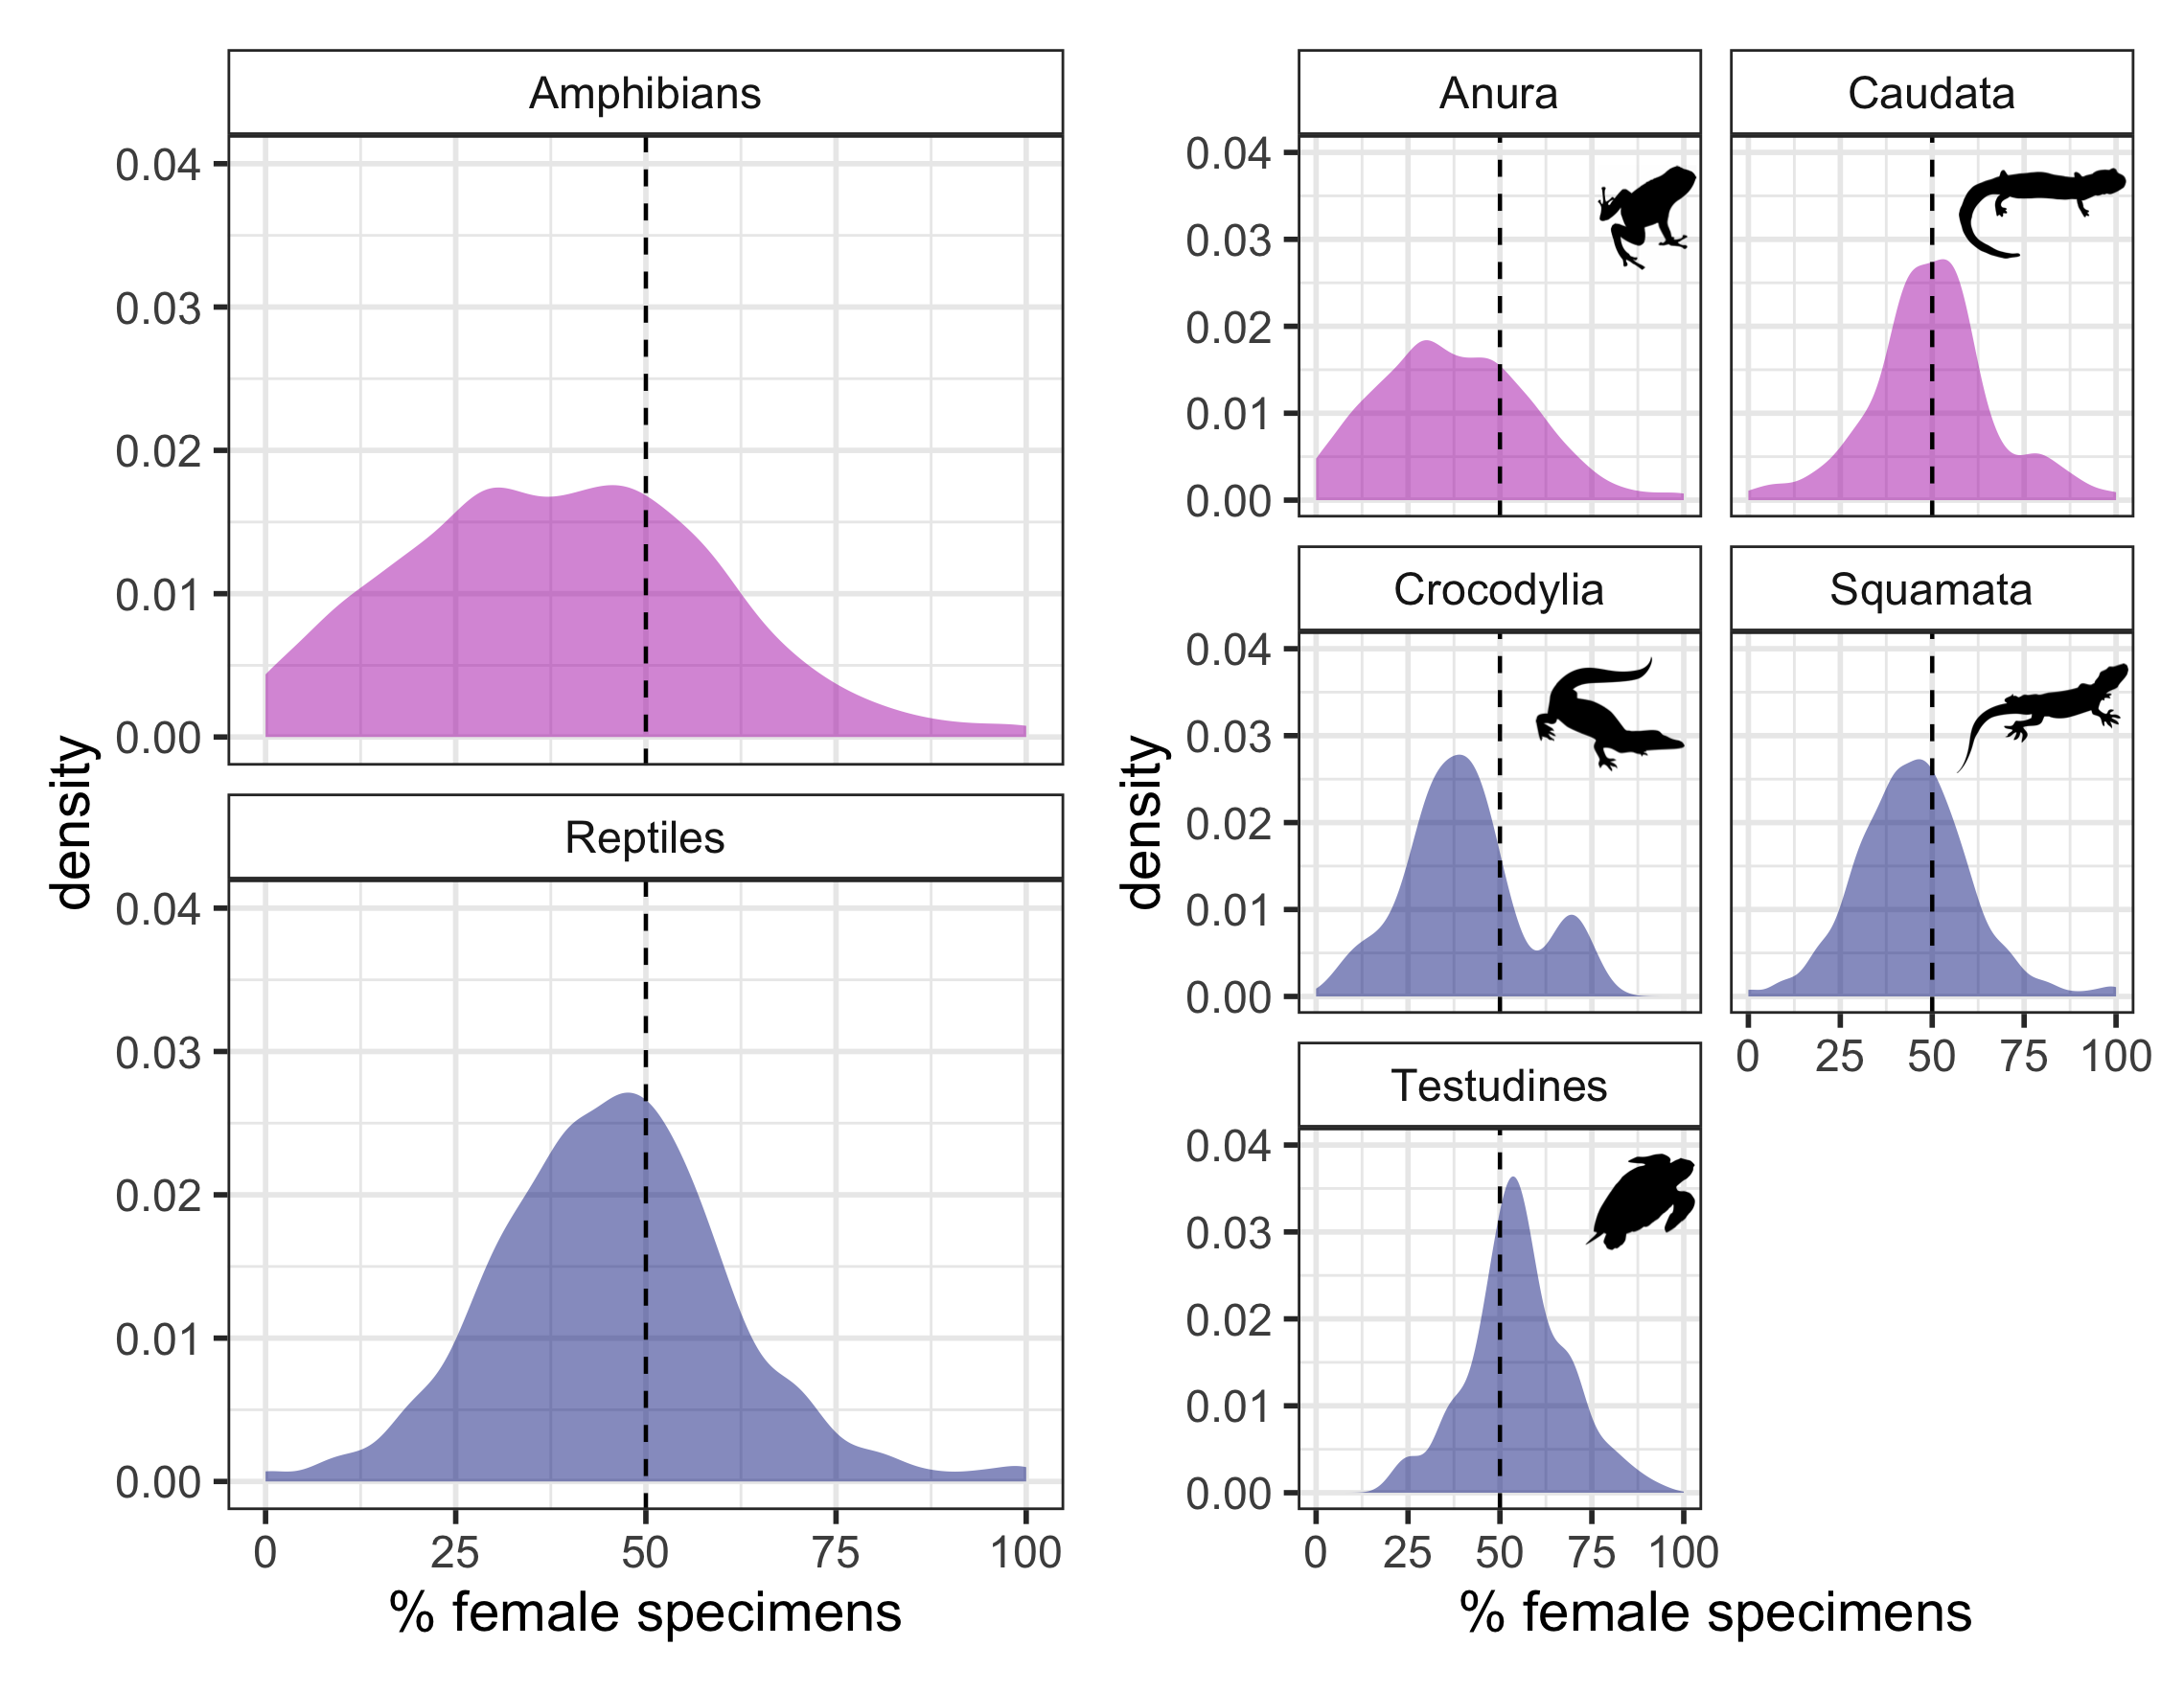
\includegraphics[width = \linewidth]{figures/class-order-density.png}
  \caption{Kernel density plots showing the \% female specimen records in each species in our dataset, for amphibians and reptiles and for each order separately. Only species with at least 10 sexed specimens are included. The dashed line represents 50\% female specimens. Silhouettes are from phylopic.org contributed by Steven Traver (frog), C. Camilo Julián-Caballero (salamander), B Kimmel (crocodile), Ghedo and T. Michael Keesey (lizard), and James R. Spotila and Ray Chatterji (turtle).}
  \label{fig-females}
\end{figure}

% figure 2
\newpage
\begin{figure}[h]
 \centering
  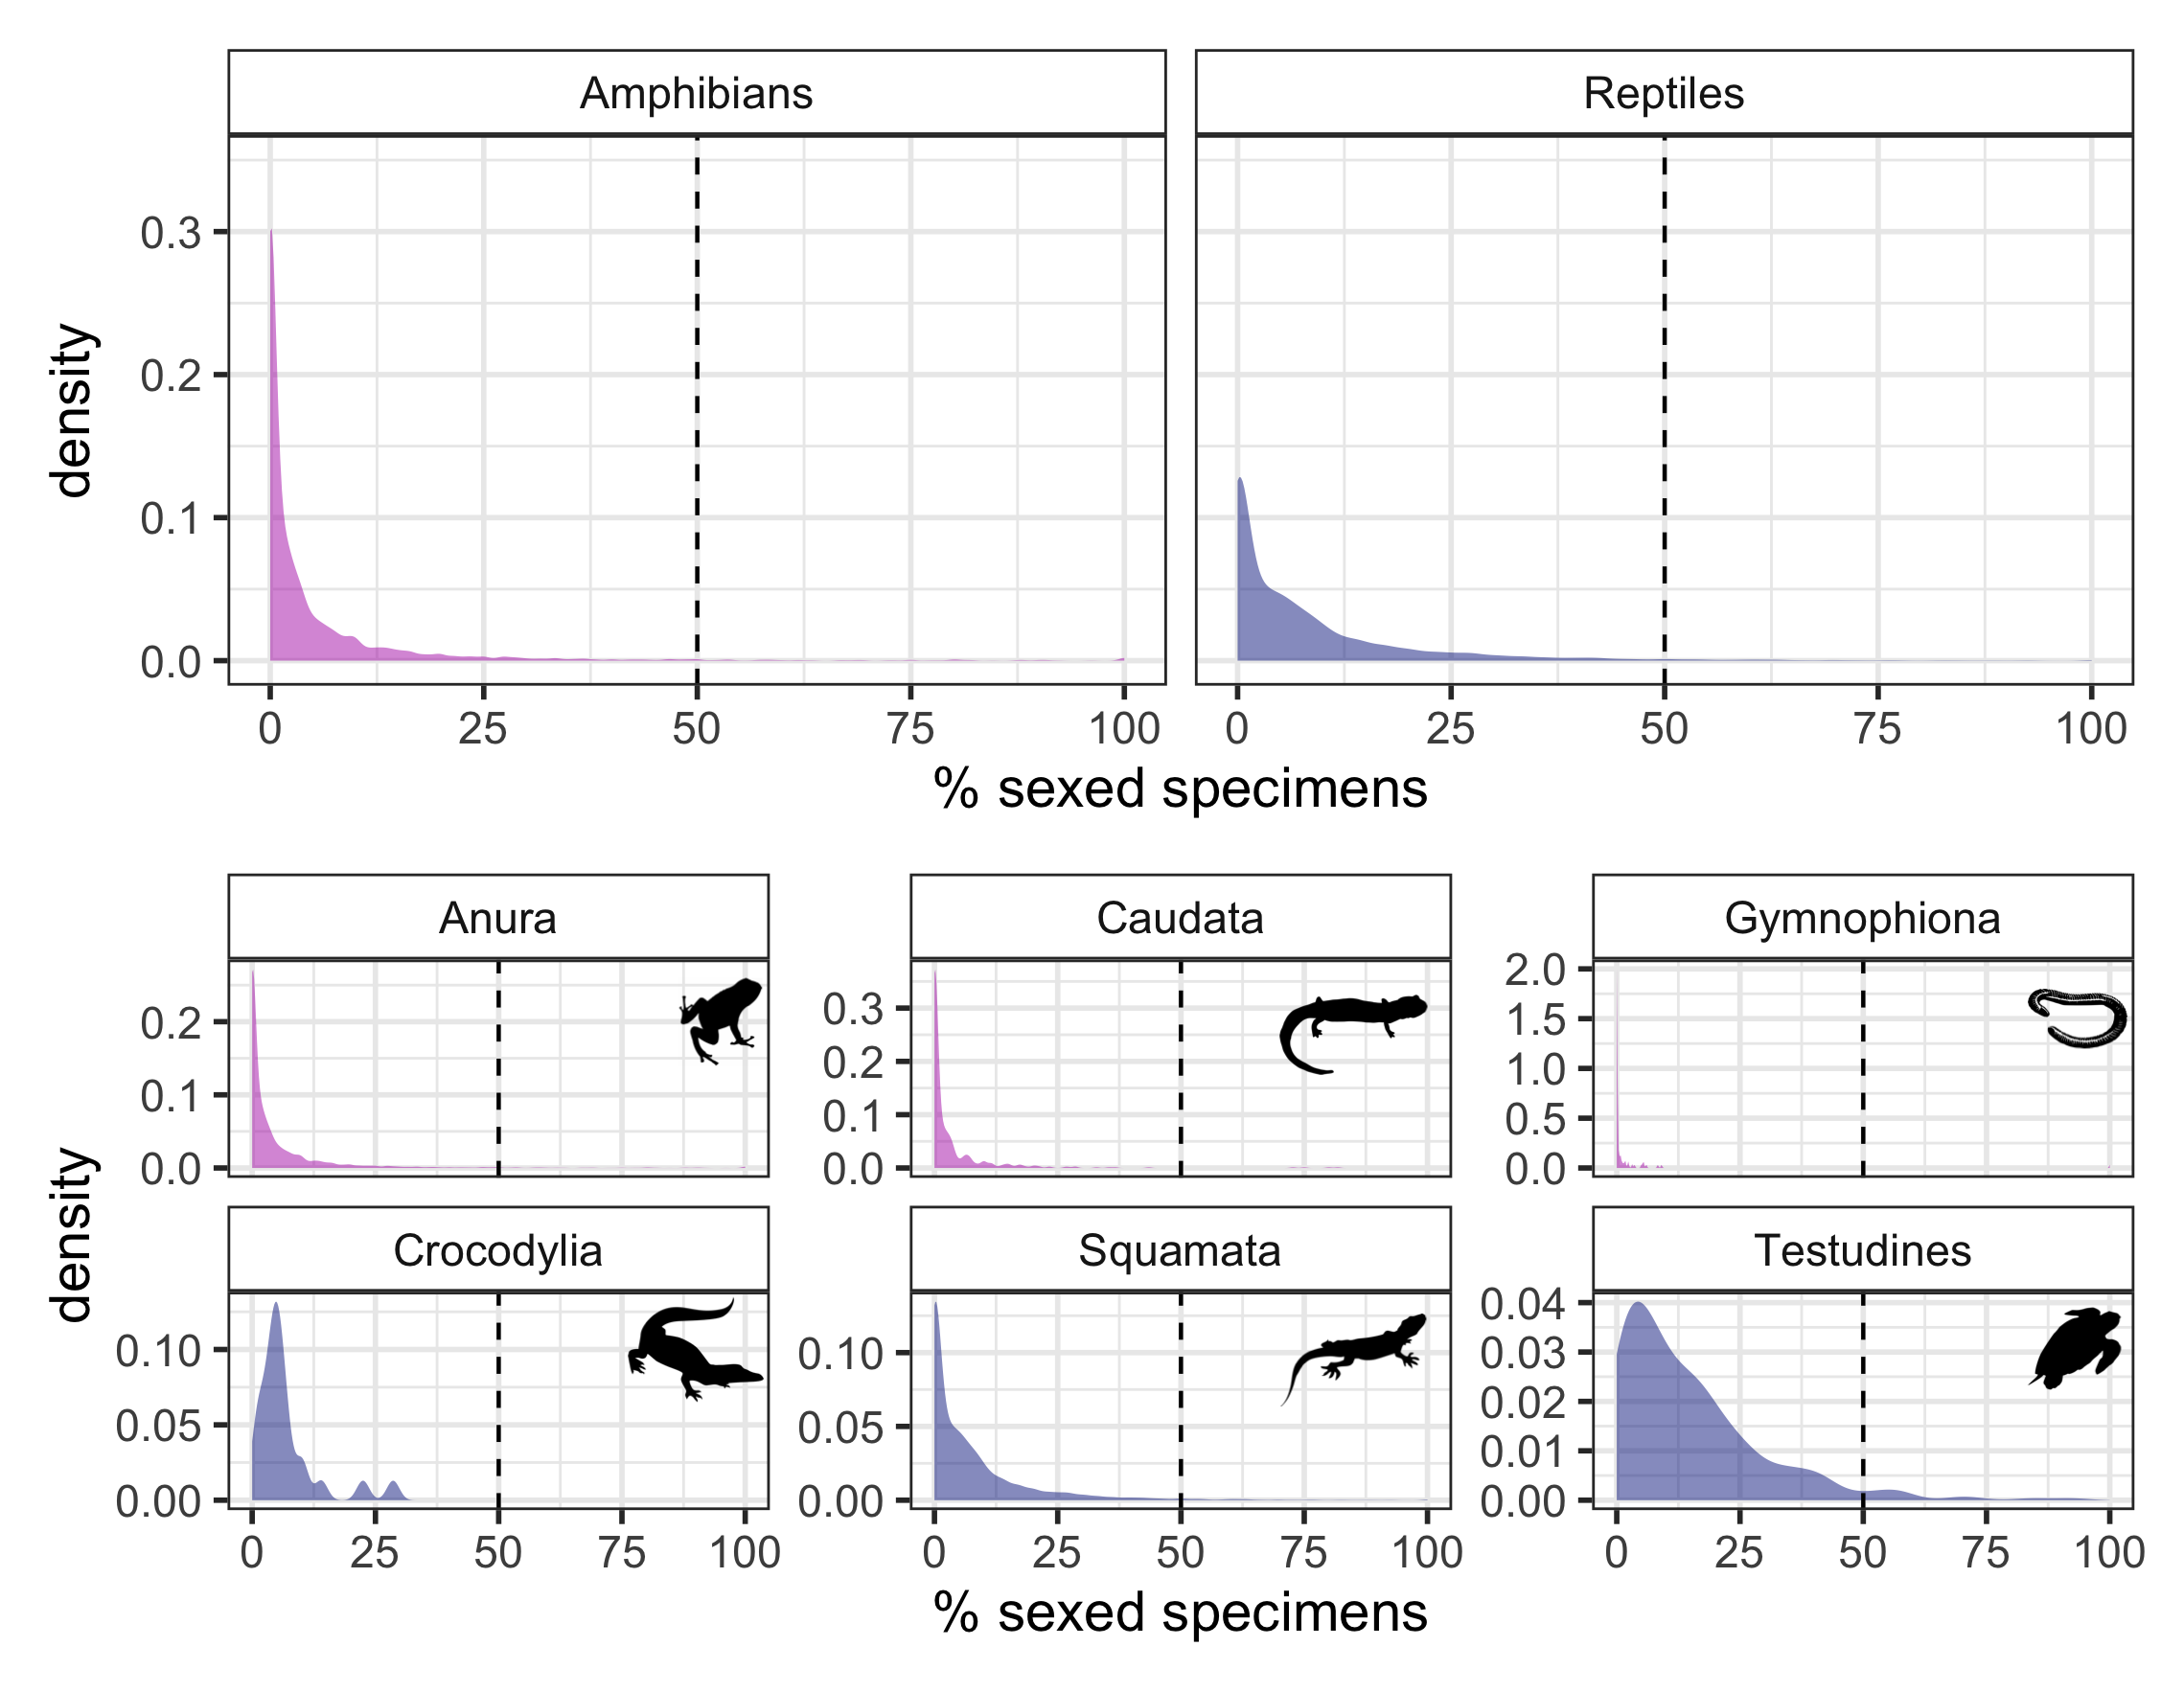
\includegraphics[width = \linewidth]{figures/unsexed-class-order-density.png}
  \caption{Kernel density plots showing the \% sexed specimen records in each species in our dataset, for amphibians and reptiles and for each order separately. Only species with at least 10 specimens are included. The dashed line represents 50\% sexed specimens. Note that the y-axis scale varies in the lower six panels. Silhouettes are from phylopic.org contributed by Steven Traver (frog), C. Camilo Julián-Caballero (salamander), Yan Wong from illustration by Charles Orbigny (caecilian), B Kimmel (crocodile), Ghedo and T. Michael Keesey (lizard), and James R. Spotila and Ray Chatterji (turtle).
}
  \label{fig-sexed}
\end{figure}


% figure 3
\newpage
\begin{figure}[h]
 \centering
  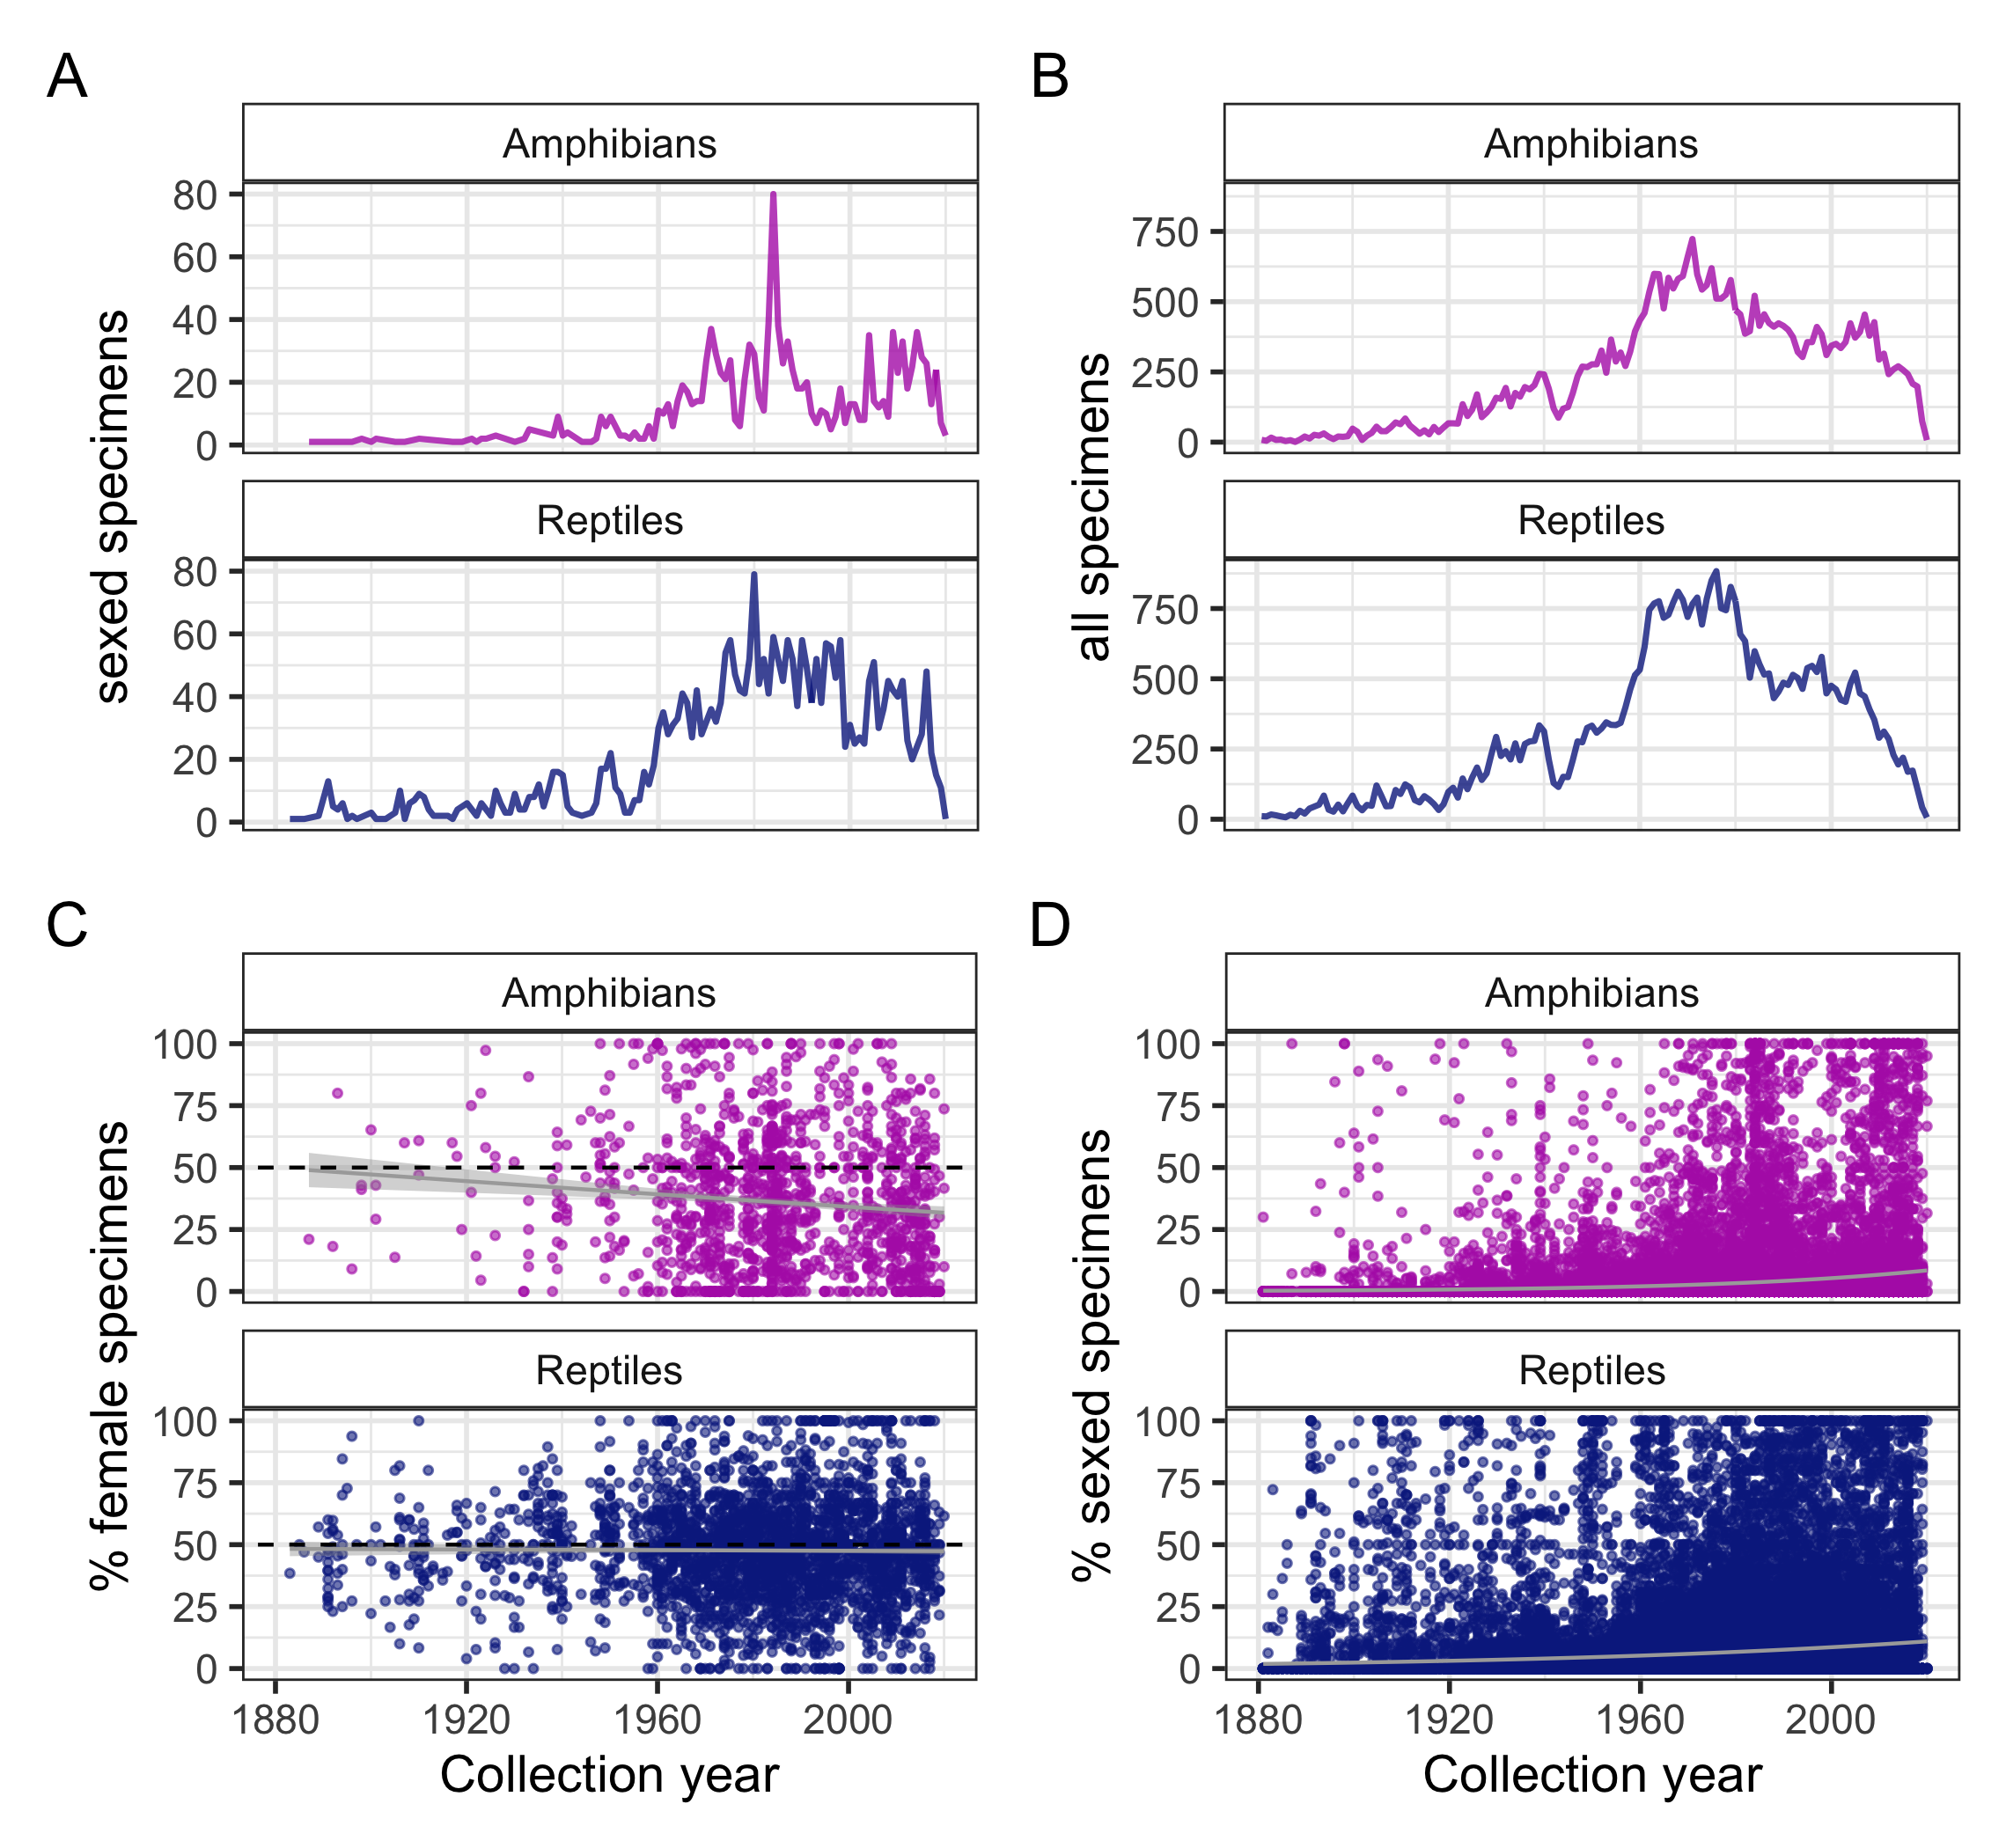
\includegraphics[width = \linewidth]{figures/years-combined-totals.png}
  \caption{Plots showing changes in the \% female or \% sexed specimen records through time in our dataset, for amphibians and reptiles. (A) Total number of female specimen records each year, and (B) total number of sexed specimen records each year. (C) \% female specimen records in each species within each year. (D) \% sexed specimen records in each species within each year. The dashed lines in (C) and (D) represent 50\% female specimens and 50\% sexed specimens respectively. Grey lines are model outputs from generalised linear models with quasibinomial errors (see Methods).}
  \label{fig-time}
\end{figure}

% figure 4
\newpage
\begin{figure}[h]
 \centering
  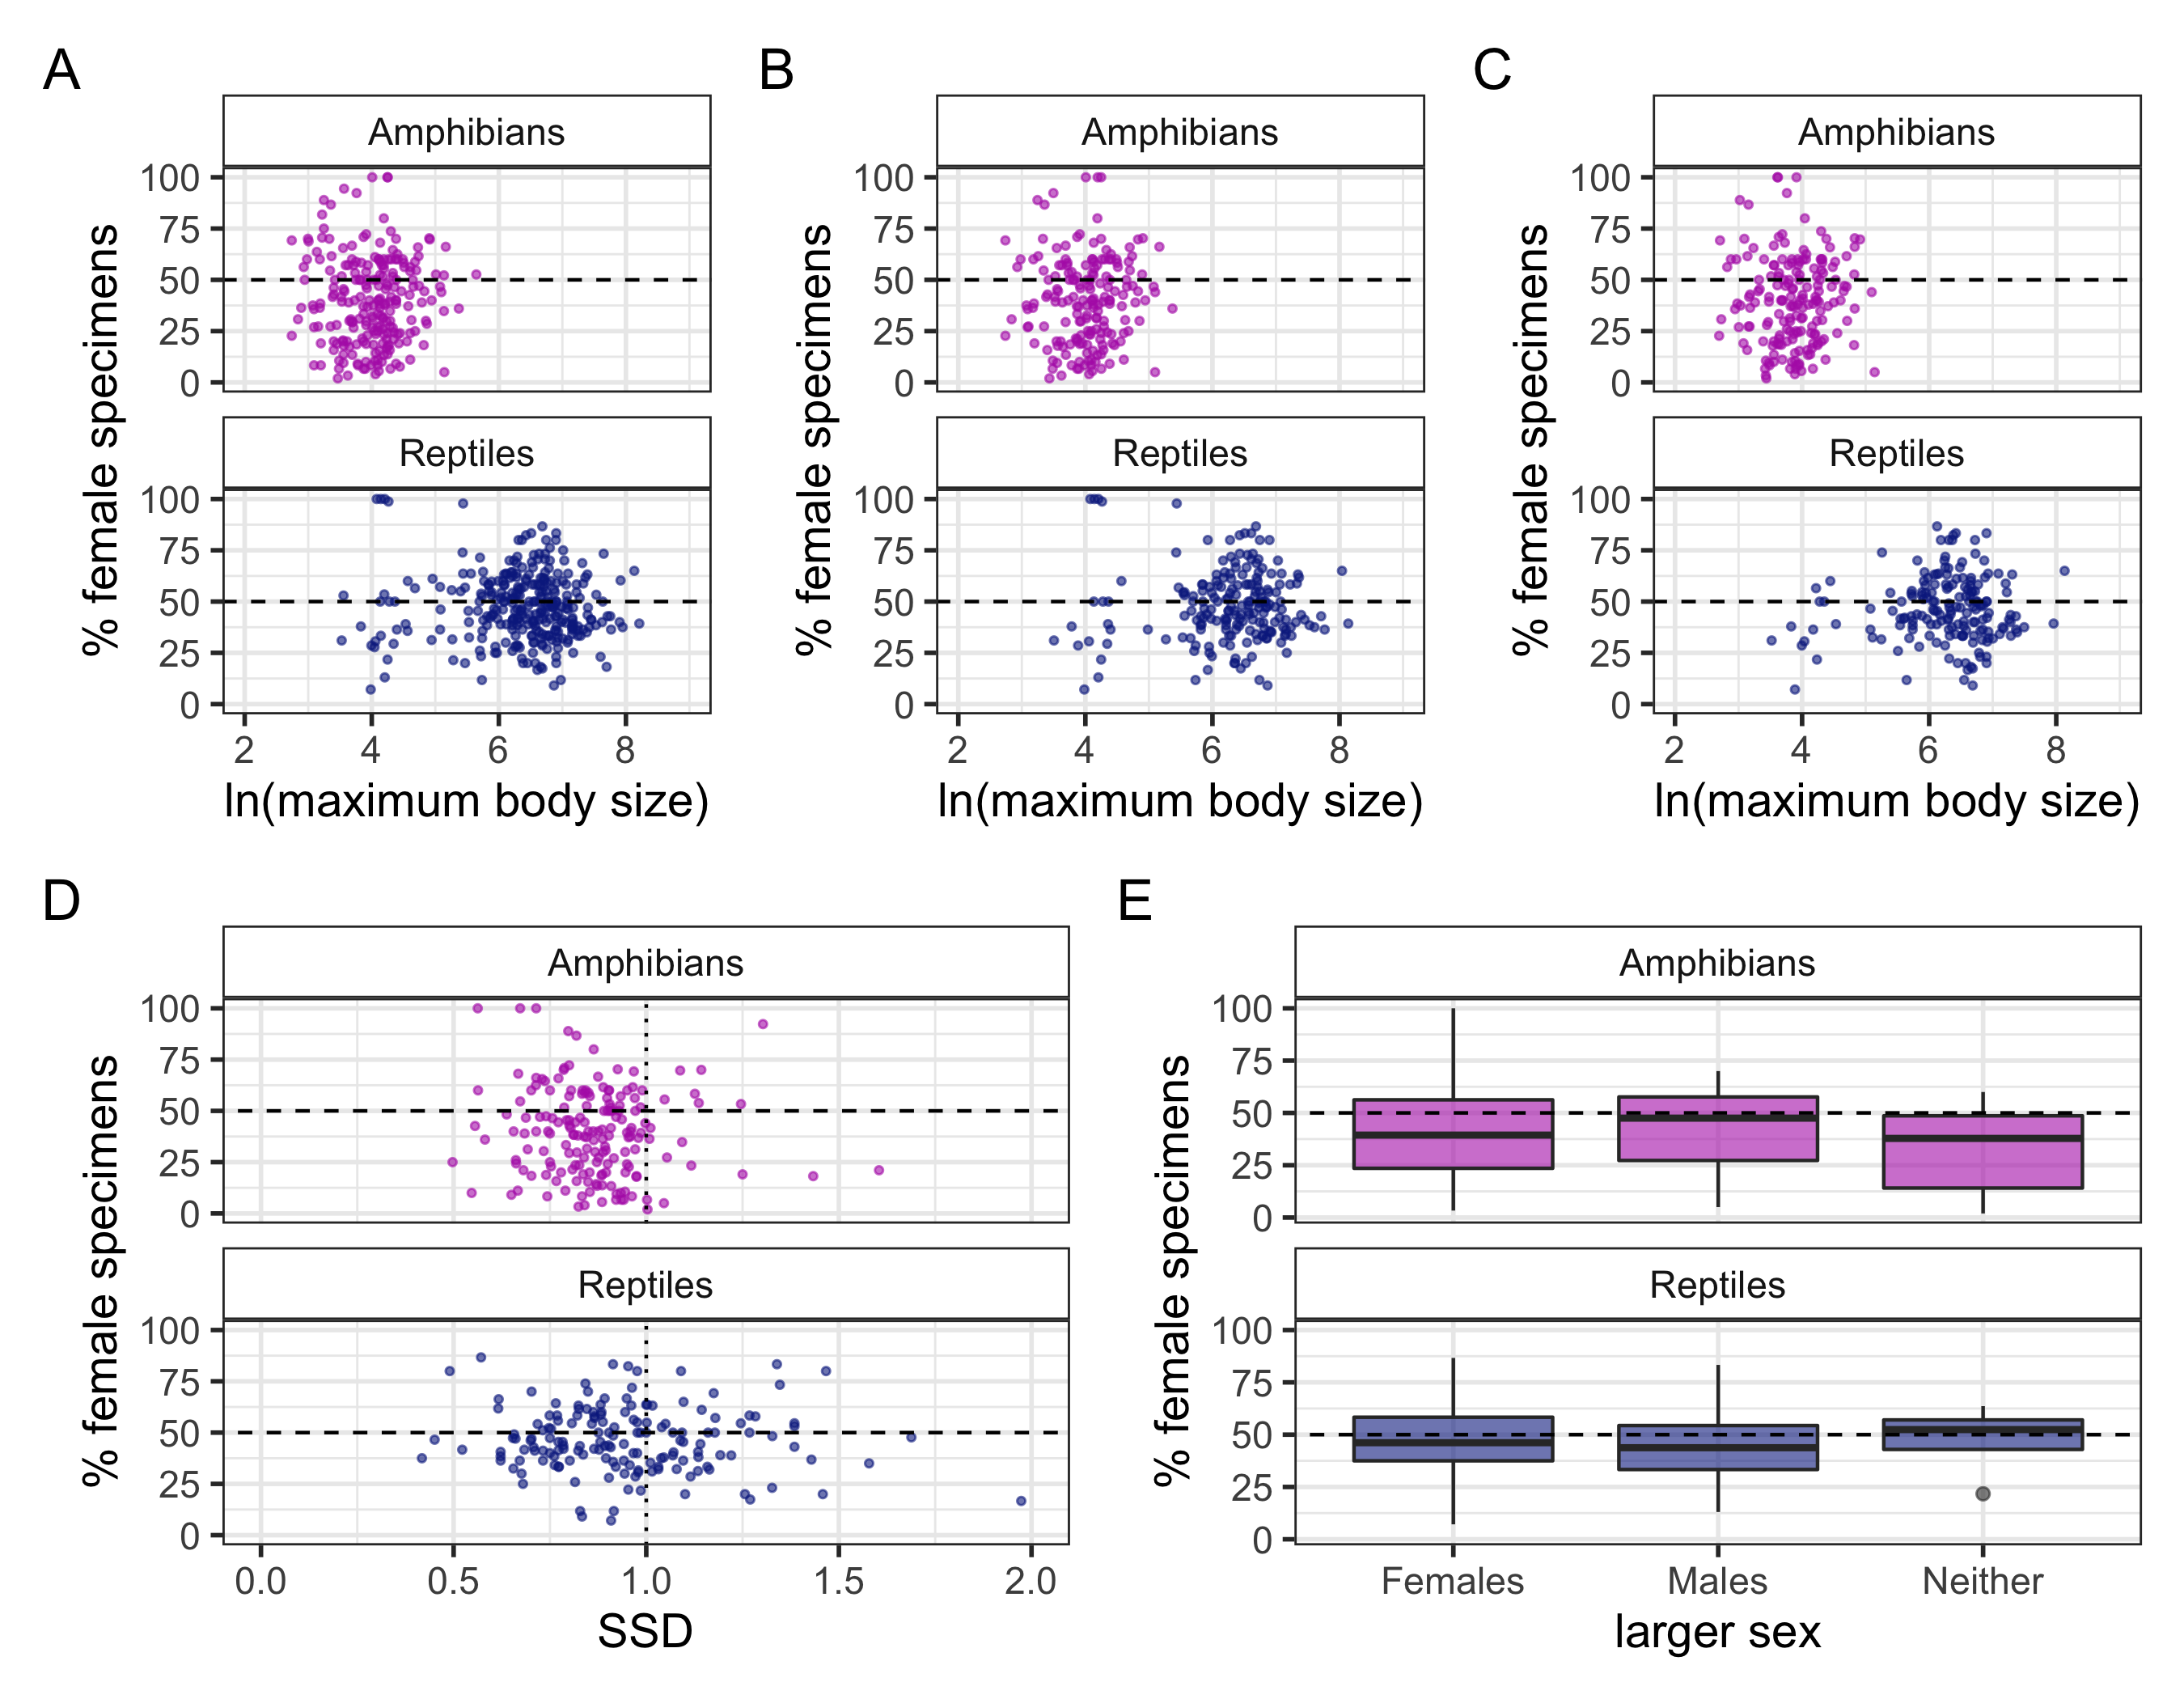
\includegraphics[width = \linewidth]{figures/size-combined.png}
  \caption{Plots showing the relationships between \% female specimen records and body size or sexual size dimorphism (SSD), for amphibians and reptiles. SSD $>$ 1 indicates species where males are larger, SSD $<$ 1 indicates species where females are larger. The x-axes in the plots are (A) overall maximum body size (mm); (B) female maximum body size (mm); (C) male maximum body size (mm); (D) SSD (male body size divided by female body size); (E) larger sex. The dashed lines represent 50\% female specimens.
}
  \label{fig-ssd-female}
\end{figure}

% figure 5
\newpage
\begin{figure}[h]
 \centering
  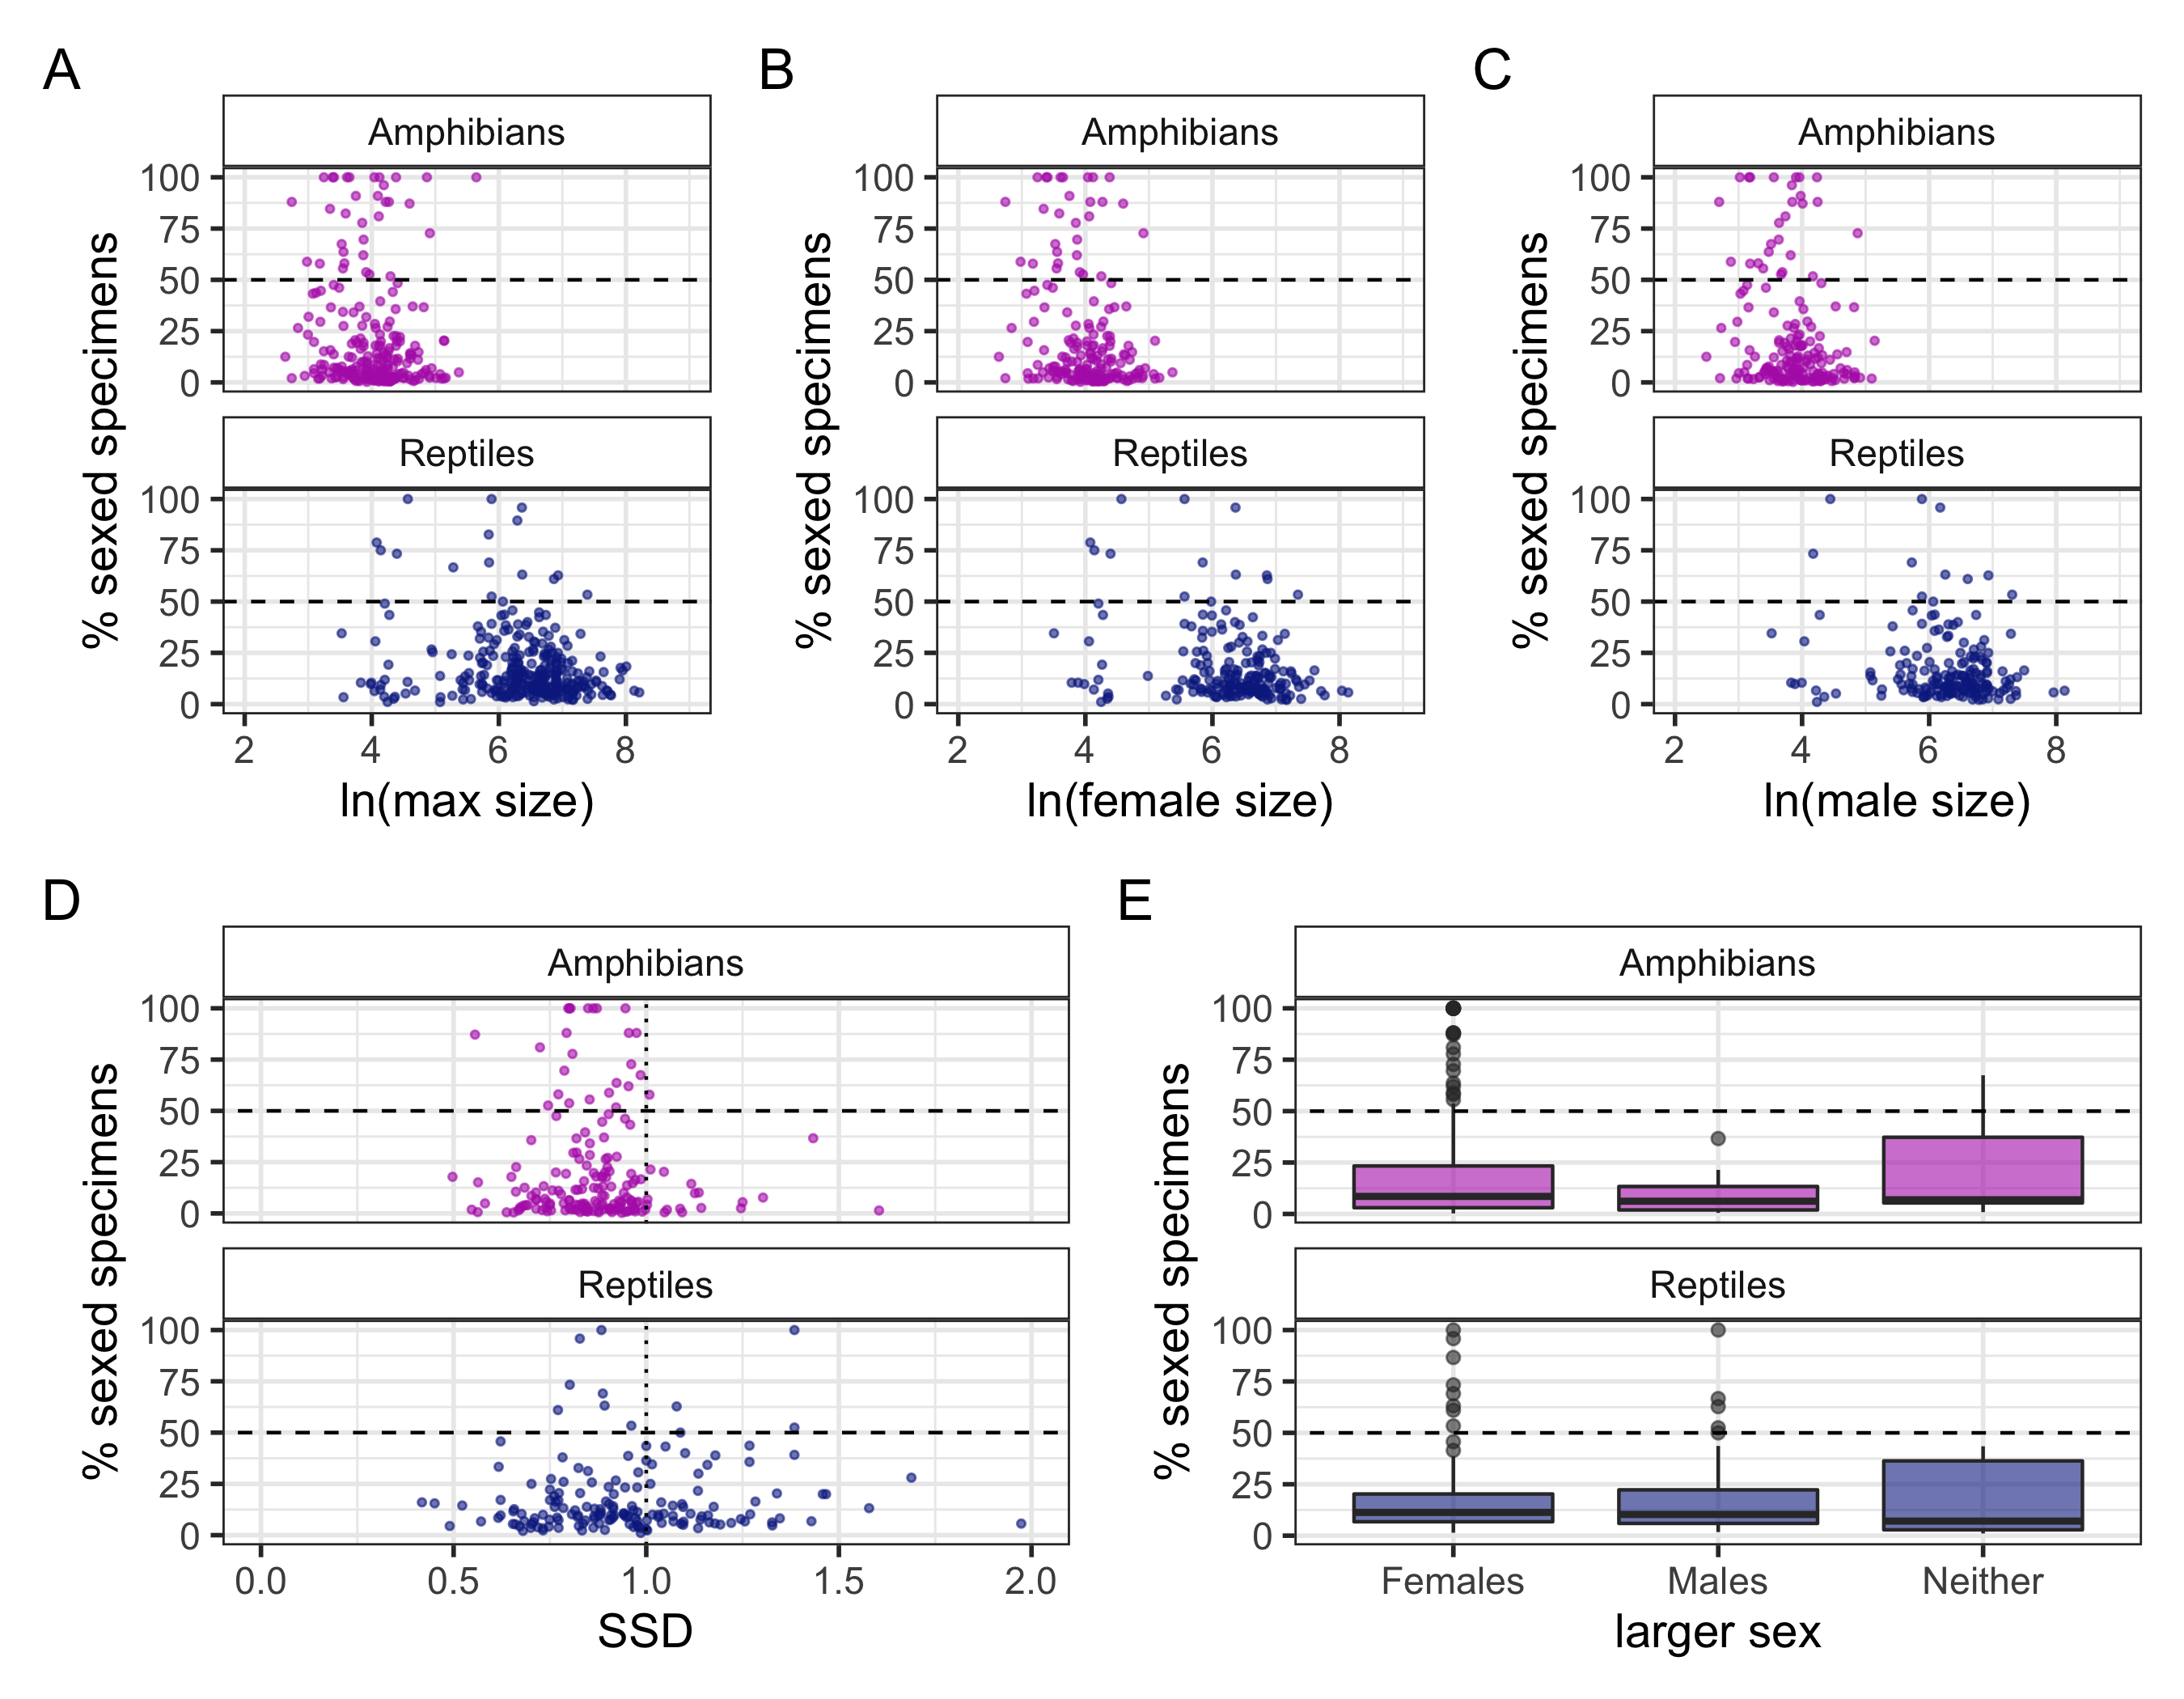
\includegraphics[width = \linewidth]{figures/size-combined-unsexed.png}
  \caption{Plots showing the relationships between \% sexed specimen records and body size or sexual size dimorphism (SSD), for amphibians and reptiles. SSD $>$ 1 indicates species where males are larger, SSD $<$ 1 indicates species where females are larger. The x-axes in the plots are (A) overall maximum body size (mm); (B) female maximum body size (mm); (C) male maximum body size (mm); (D) SSD (male body size divided by female body size); (E) larger sex. The dashed lines represent 50\% sexed specimens. 
}
  \label{fig-ssd-sex}
\end{figure} 

\end{document}